\chapter{Representing Information for GDPR Compliance using Ontologies}
\label{chapter:vocabularies}

This chapter presents OWL2 ontologies developed to fulfil research objective $RO3$ defined in \autoref{sec:intro:RO} regarding representation of information.
The chapter first presents a more detailed description of the methodology in \autoref{sec:intro:ontology-engineering} regarding developing and evaluating ontologies based on summary presented earlier in \autoref{sec:voc:methodology}.
It then presents the ontologies of: (i) GDPRtEXT (\autoref{sec:voc:GDPRtEXT}) which provides a linked data representation of GDPR text and a glossary of GDPR compliance concepts, and which satisfies research objective $RO3(a)$ by providing an ontological representation of concepts and text of GDPR; (ii) GDPRov \autoref{sec:voc:GDPRov} which enables representing provenance of activities associated with personal data and consent in ex-ante and ex-post phases, and fulfils research objective $RO3(b)$; and (iii) GConsent (\autoref{sec:voc:GConsent}) which enables representing information regarding consent, and fulfils research objective $RO3(c)$.

Each ontology is presented with a summary of its motivation, engineering process, and dissemination. Ontologies are presented with their evaluation based on the extent to which they satisfy the competency questions used in their development and through comparison with analysed approaches in state of the art in \autoref{sec:sota:analysis}.

In addition to these, Data Privacy Vocabulary (DPV), initially presented in \autoref{sec:intro:dpvcg}, is also included as an external contribution of the thesis based on work done by author of this thesis within the W3C Data Protection Vocabularies and Controls Community Group (DPVCG), and overlap of DPV with the research presented. \autoref{sec:voc:DPV} presents an overview of DPV and compares it with GDPRtEXT, GDPRov, and GConsent - and demonstrates their similarity in representing information while drawing attention to distinguishing features.
The section also presents a comparison of DPV with state of the art as identified in \autoref{chapter:sota}.

\section{Methodology for Ontology Engineering}\label{sec:voc:methodology}

\subsection{Utilisation of Existing Ontology Engineering Methodologies}
The creation of ontologies followed guidelines and methodologies deemed `best practice' by semantic web community. In this, `Ontology development 101: A guide to creating your first ontology' by Noy and McGuiness \cite{noy_ontology_2001} was utilised as a guiding document for ontology creation. It provided steps for construction of an ontology with attention on avoiding bad design decisions and common pitfalls. It also suggested use of competency questions to determine scope of an ontology and for evaluation after creation.
% For this, the compliance questions presented in \autoref{} were used as competency questions.
The guide suggested Protégé\footnote{\url{https://protege.stanford.edu/}} - a popular and widely adopted tool - for ontology development as it supports semantic reasoners to detect logical inconsistencies arising from asserted facts and axioms in ontology.
Use of this guide provided a foundational basis for initiating the ontology development process and for using compliance questions from \autoref{sec:info:compliance-questions} as competency questions to identify concepts and relationships, testing for inconsistencies using Protégé, and iteratively building an ontology. 

The development of ontologies followed a combination of NeOn methodology \cite{suarez-figueroa_neon_2012} and UPON Lite methodology \cite{de_nicola_lightweight_2016}. NeOn provides a flexible workflow for ontology development through use of scenarios such a using a specification, reusing and re-engineering existing ontological and non-ontological resources, and utilisation of ontological design patterns. 
UPON Lite is a lightweight methodology for rapid ontology engineering that was used in combination with NeOn for iteratively developing ontologies in an agile fashion. UPON Lite consists of six steps: identification of domain terminology, construction of domain glossary, creating a taxonomy, predication as properties, meronymy for complex components, and conceptualisation into an ontology.
The combination of NeOn and UPON Lite consisted of identifying development scenarios and specifying them as requirements using NeOn, then using UPON Lite to derive actionable tasks and implementing ontology creation.

The methodology used to develop ontologies presented in this chapter explicitly specifies competency questions used to derive its concepts based on compliance questions from previous chapter (\autoref{sec:info:compliance-questions}). This approach enables tracing lineage of a concept to its role in compliance process and provides transparency in development process.
To compare methodology used in this thesis with other methodologies used to develop ontologies within relevant approaches in SotA - some utilise legal experts which act as domain experts to validate developed ontologies and their interpretation - such as in research projects SPECIAL and MIREL (see \autoref{sec:sota:gdpr-semweb}). Such projects involve commercial partners who provide real-world use-cases and data to inform and evaluate developed research.
Others - such as Ujcich et al. \cite{belhajjame_provenance_2018} - interpret GDPR as a set of requirements for compliance in their modelling of information. In either case, approaches within SotA do not provide competency questions that could be used to develop ontologies\footnote{Deliverables of research project provide a description of how the concepts of their ontologies were developed from legal requirements, but such descriptions are argumentative and limited to the specified domain or use-case, and hence do not provide a concrete requirement that can be used to develop an ontology to answer the compliance questions.}.

% The aims and motivations of this thesis (see \autoref{sec:intro:background}) are based on representing information for assisting the compliance process rather than an evaluation of compliance itself. Therefore, the research has been documented methodologically to indicate its aims, motivations, methodology, and resources used to shape conceptualisations and rationalisations, and published in an open and accessible manner to enable transparency and reuse.

\subsection{Ontology Quality}
The quality of an ontology refers to quality of its design of concepts and relationships, and quality as a semantic dataset. While following a suitable ontology engineering methodology provides a structured ontology, it still needs to be inspected for quality in terms of ontology as well as for intended use-cases and scenarios. For this, existing publications \cite{gurk_towards_2017,vrandecic_ontology_2010} list various methods of ontology quality detection, evaluation, and suggest solutions to fix identified problems.

OOPS!\footnote{\url{http://oops.linkeddata.es/}} \cite{poveda-villalon_oops!_2014} is a useful tool for ontology evaluation which detects common pitfalls in design of concepts and relationships and provides a documented output which can be persisted for provenance of ontology development. Each pitfall detected by OOPS! is categorised along structural, functional, and usability-profiling dimensions. The tool also provides an indicative measure of importance regarding pitfalls in terms of critical, important, and minor levels.
OOPS! was used for detecting catalogued common pitfalls in evaluation of developed ontologies. Identified pitfalls were corrected by changing underlying relationships to remove them. 

Quality was also assessed and maintained by asserting sufficiency of developed ontology to represent and query information based on collected use-cases presented in \autoref{sec:info:use-cases}. In this process, missing concepts and relationships were added to the ontology, while incorrect ones were removed or rectified.
 % Where existing models were found to be insufficient or incorrect, these were rectified by either removing the offending parts or re-designing them - based on its impact on compatibility with previous versions.

\subsection{Ontology Documentation}
Ontology documentation was created by using WIDOCO\footnote{\url{https://dgarijo.github.io/Widoco/}} \cite{garijo_widoco_2017} - a tool which uses ontology metadata to create HTML documents listing its classes and properties. Ontology metadata consists of information regarding the ontology as well as its concepts and properties integrated into its serialisation as annotations. WIDOCO provides a document of suggested metadata indicating best practices for ontology documentation. It builds upon LODE\footnote{\url{http://www.essepuntato.it/lode}} which is itself a popular ontology documentation service.

The output of WIDOCO is a HTML document along with various serialisations of ontology for content negotiation that can be published and used as an online resource. Additional information was manually added to HTML documentation to specify aims and methodologies used in development of ontologies as well as examples of use-cases and diagrams intended for human consumption. WIDOCO integrates OOPS! to detect pitfalls and documents the output. It also provides an interactive visualisation of the ontology using WebVOWL\footnote{\url{http://vowl.visualdataweb.org/webvowl.html}}.

\subsection{Dissemination}
The ontologies were published on internet using a stable IRI through persistent identifiers on servers hosted by ADAPT Research Centre\footnote{\url{https://adaptcentre.ie/}} and School of Computer Science \& Statistics\footnote{\url{https://scss.tcd.ie/}} within Trinity College Dublin. Initially, persistent identifiers were provided using purl\footnote{\url{https://purl.org/}} which later had issues regarding maintenance and frequent problems with URL resolution. The ontologies were then modified to utilise W3ID\footnote{\url{w3id.org/}} persistent identifiers maintained by W3C Permanent Identifier Community Group\footnote{\url{https://www.w3.org/community/perma-id/}}. The ontologies published in this manner followed best practices and principles related to use of Linked Open Data\footnote{\url{https://www.w3.org/TR/ld-bp/}}, Linked Open Vocabularies\footnote{\url{https://dgarijo.github.io/Widoco/doc/bestPractices/index-en.html}}, and FAIR\footnote{Findability, Accessibility, Interoperability, and Reusability (FAIR) \url{https://doi.org/10.1038\%2Fsdata.2016.18}} principles.

Each ontology was added to Linked Open Vocabularies\footnote{\url{https://lov.linkeddata.es/}} (LOV) - a community listing that catalogues vocabularies in semantic web community. Each ontology was published in Zenodo\footnote{\url{zenodo.org/}} which provides open repositories and assigns a unique DOI to repositories. The ontology and its resources were also added to public hosting repositories such as GitHub\footnote{\url{github.com/}} and an instance of OpenGogs\footnote{\url{opengogs.adaptcentre.ie/}} hosted on institution servers. Each ontology was published under an open and permissive license (CC-by-4.0\footnote{\url{https://creativecommons.org/licenses/by/4.0/}}) to promote its use and adoption.

\subsection{Evaluation}
Evaluation was carried out by analysing sufficiency of each ontology to represent information for answering competency questions. This was carried out in an iterative manner where each iteration consisted of developing the ontology, evaluating it, and utilising results of evaluation as feedback to identify areas of improvement such as missing concepts and relationships or incorrect assumptions.

The ontology was also evaluated against common pitfalls using OOPS! as described earlier regarding ontology quality. The OOPS! ontology report is published along with ontology documentation, and can be manually generated by using OOPS! online service. Documentation and publishing standards were evaluated by assessing whether ontologies met existing criteria advocated by the community (such as 5-star principle for linked data \footnote{\url{https://5stardata.info/en/}} and FAIR principles). Finally, each ontology was published and presented in a peer-reviewed venue and publication, with more information about publications provided in the respective ontology's section.

Evaluation of work as a research contribution was carried out based on whether it satisfied its research objectives motivating its development and whether it provided novel contributions compared to existing approaches within state of the art. The details of this are presented in evaluation sections of each ontology.

\subsection*{Summary of Methodology}
Based on above description of ontology engineering processes, the methodology used for ontology engineering and development is summarised through as:
\begin{enumerate}
    \item \textbf{Identification of aims, objectives, scope:} The first step was to identify aim and objectives of information to be represented, followed by deciding on scope regarding relation to GDPR compliance. For ontologies presented in this chapter, aims and objectives are listed in \autoref{sec:intro:RQ}. % introduction
    \item \textbf{Identify and analyse relevant information:} Using identified scope, relevant information was gathered from various sources including authoritative, community, and publications - and analysed to identify terms of importance and requirements regarding GDPR compliance. The information is presented as background of GDPR in \autoref{sec:background:GDPR} and analysed with regards to compliance in \autoref{chapter:information}.
    \item \textbf{Create use-cases and competency questions:} From the analysed information, different use-cases were identified to better understand application of information in compliance scenarios and  requirements of different stakeholders in this process. This was done using information interoperability model presented in \autoref{sec:info:model}. The analysed information was used to create compliance questions, as presented in \autoref{sec:info:compliance-questions}, which identify relevant information for evaluation of compliance. These compliance questions were utilised as competency questions in development and evaluation of ontologies.
    \item \textbf{Identify concepts and relationships:} Relevant concepts and relationships were identified to express information required to answer compliance questions in identified use-cases. This was an iterative and cyclic process where identified concepts and relationships were re-purposed to better suit some design pattern or compliance requirements.
    \item \textbf{Create Ontology:} The identified concepts and relationships were formalised as an ontology in OWL2 using the Protégé ontology development environment. In this process, a semantic reasoner (i.e. Pellet\footnote{\url{https://github.com/stardog-union/pellet}} and HermiT\footnote{\url{http://www.hermit-reasoner.com/}}) was used to identify logical inconsistencies in ontology. Minor inconsistencies were fixed by changing appropriate relationships between concepts, while major inconsistencies required evaluation of information identified in step 4. Development of ontology utilised best practices advocated by semantic web community in terms of ontology metadata, documentation, design patterns, publication, and dissemination.
    \item \textbf{Evaluate:} The ontology was evaluated for sufficiency towards representing information for answering competency questions. The use of a semantic reasoner detected logical inconsistencies in expressed facts and axioms, while OOPS! provided detection of common pitfalls and bad design patterns.
    The quality of metadata and documentation was evaluated in terms of sufficiency based on community guidelines. Where an ontology was published and/or presented as a resource or as part of a peer-reviewed publication, resulting comments and feedback were used to identify areas of improvement. Citations of ontologies and associated publications were used to identify criticisms (if provided) and to compare them with work presented in citing publication.
    \item \textbf{Dissemination:} The ontology and its documentation were published online with a persistent identifier as a FAIR resource with an open and permissive license. This included publication of ontology, datasets, and code in a public repository accompanied by human-readable documentation about its creation and utilisation.
    \item \textbf{Progressive iterations:} Within a single iteration of development, an ontology was created and evaluated by following steps 2 to 6. Multiple iterations consisted of repeating these steps as in an development cycle to progressively improve the ontology by adding new concepts or removing existing undesirable ones. Previous versions of ontology were retained with their documentation for provenance where possible to indicate milestones in its development.
\end{enumerate}

% \subsection*{Modularity of Ontologies}
% The research question stated in \autoref{sec:intro:RQ} lays the scope for the work of developing an ontological re{}presentation of information associated with GDPR compliance and concerning activities associated with processing of personal data and consent.
% This information is identified through the research objectives $RO1$ and $RO2$.
% They provide the analysis of GDPR and the compliance questions as presented in \autoref{chapter:information} which act as requirements in the ontology engineering process.
% This directly provides the objective of developing an ontology to represent information about processing of personal data and consent.

\section{GDPRtEXT - Linked Open Dataset of GDPR text \& Glossary of Concepts}\label{sec:voc:GDPRtEXT}

This section describes the GDPRtEXT ontology and dataset which provides a linked data version of text of GDPR and a SKOS glossary of concepts associated with its compliance. The section presents the motivation and creation of GDPRtEXT, its publication, dissemination, and comparison with relevant approaches in state of the art. The latest iteration of GDPRtEXT (v0.6) is available online\footnote{\url{https://w3id.org/GDPRtEXT/}} with its documentation and code repository\footnote{\url{https://github.com/coolharsh55/GDPRtEXT/}}.

\subsection{Motivation}
GDPR as a legislation consists of text which is structured into 173 Recitals, 99 Articles (further grouped into Chapters and Sections), and 21 Citations. Each Article may have one or more Paragraphs which itself may have one or more Sub-Paragraphs. As per norms used in legislations, each individual clause - whether an article, paragraph, or sub-paragraph - is identified with an alphanumeric number as provided. These are commonly referenced in textual notation as identifiers, for example \textit{Article 8 Paragraph 2 Sub-Paragraph c} can be referred to as: \textit{A8(2-c), A(8-2c), A8-2(c), Art.8 2(c), Art-8-2-c}. As there is no standard or accepted commonality in specifying such references, and because such notations are intended for human readability and interpretation - a strict set or specification of notations does not exist. This presents difficulty when representing such information in machine-readable formats.

The EU Publications Office currently publishes legislation metadata at document level which provides information about GDPR as a legislation using  ELI ontology and standard \cite{thomas_european_2019} but does not specify granular information about its contents - such as its articles. The EU Publications Office has indicated its intention to provide such granular metadata in future (see footnote in \autoref{sota:analysis:representation}).
Currently, concepts arising from legislations as well as those used in context of GDPR compliance have no standardised reference to provide commonality between two representations in different use-cases. 

Within the larger scope of legal compliance, information is always associated with clauses and concepts of a law - in this case GDPR.
Amongst approaches part of SotA presented in \autoref{chapter:sota}, only two approaches consider association of information with GDPR within scope of their work as presented in \autoref{sota:analysis:representation}.
Other approaches, where they reference concepts and clauses of GDPR, do so in an ad-hoc manner using textual notations such as ``Article 4-11''.
As the analysis in \autoref{sota:analysis:representation} points out, the two approaches modelling clauses of GDPR have three drawbacks - (a) the representation is incompatible with ELI ontology, (b) none provide a glossary of terms relevant for compliance, and more importantly (c) neither resource can be reused as it is not published in an open and accessible manner.
Addressing this gap is required to fulfil research objectives related to linking of information with GDPR.

With this motivation research objective $RO3(a)$ was established in \autoref{sec:intro:RO} and is fulfilled by GDPRtEXT - which provides an OWL2 ontology for granular representation of GDPR text and a dataset created using this ontology for a linked data representation of GDPR where each clause has a unique IRI.
GDPRtEXT also provides a SKOS glossary of terms associated with compliance and links them with their definition and relevance to clauses within GDPR using the developed ontology. 
It thus enables linking of information with specific clauses and concepts of GDPR.

\subsection{Ontology Engineering and Creation of Resource}\label{sec:voc:gdprtext-engineering}
Following the methodology described in \autoref{sec:voc:methodology},  development of competency questions was based on understanding and analysis of how legal articles are referenced in text in relation to compliance.
Competency questions presented here are categorised based on whether they concern structure of GDPR or representation of concepts associated with compliance. These competency questions investigate structure and concepts of GDPR as a document and thereby differ from compliance questions presented in \autoref{chapter:information} which are concerned with investigating information for compliance. The competency questions for GDPRtEXT are outlined below with identified requirements:

\subsubsection{Structure of GDPR text}
\begin{enumerate}[label={\texttt{CQ.\theenumi}}]
    \item How many Recitals are there within GDPR?
    \item How many Chapters are there within GDPR?
    \item How many Sections are there within GDPR?
    \item How many Articles are there within GDPR?
    \item How many Paragraphs are there within GDPR?
    \item How many Sub-paragraphs are there within GDPR?
    \item How many References or Citations are there within GDPR?
    \item Article 4 belongs to which Chapter? (generalised to which \textit{Chapter} does \textit{Article X} belong?)
    \item Which clause contains the definition of 'personal data'? (generalised to definition of \textit{concept X})
    \item What is the structural hierarchy of the document?
    \item What are the `Principles' defined in GDPR? (generalised to \textit{conceptA} with types \textit{conceptB}, e.g. `Accountability' as a type of `Principle')
    \item Which articles, paragraphs, and sub-paragraphs are relevant to the validity of given consent? (generalised to relevant to \textit{concept X})
    \item How to associate information regarding given consent to relevant clauses in the GDPR? (generalised to association information regarding \textit{concept X})
    \item How to associate information regarding compliance to a specific article of the GDPR?
\end{enumerate}

Based on these, following requirements were identified with regards to extending the existing ELI ontology:
\begin{itemize}
    \item Structure of text must be specified with granularity and a hierarchy of Document, Chapter, Section, Article, Paragraph, Sub-Paragraph along with Recitals and Citations.
    \item Relations between clauses must be specified e.g. Paragraph belongs to an Article.
    \item Relations must be transitive e.g. Paragraph in an Article must also be in the Article's Chapter.
    \item Each individual clause must have a unique IRI to enable linking of information to it.
\end{itemize}

\subsubsection{Concepts associated with GDPR compliance}
\begin{enumerate}[label={\texttt{CQ.\theenumi}},resume]
    \item What type of data does the GDPR define?
    \item What types of consent does the GDPR define?
    \item What are the different entities referred to within GDPR?
    \item Which activities are associated with processing of personal data?
    \item Which activities are associated with consent?
    \item What are the conditions or criteria associated which affect sensitivity of processing?
    \item What activities are relevant to a data breach?
    \item Which activities are relevant regarding compliance?
    \item What are the principles defined in GDPR?
    \item What are the rights provided by the GDPR?
    \item Which criteria does the GDPR mention for right to data portability?
    \item Which criteria does the GDPR mention for right to be informed?
    \item What are the obligations mentioned within GDPR?
    \item What are the obligations of the Controller?
    \item What are the obligations of the Processor?
    \item What are the obligations of a DPO?
    \item What are the lawful basis for processing of personal data specified in the GDPR?
    \item What are the conditions for valid consent under GDPR?
    \item Which obligations are mentioned in relation to data collection?
    \item Which obligations are mentioned in relation to obtaining consent?
    \item Which obligations are mentioned in relation to retaining personal data?
    \item Which obligations are mentioned in relation to security of personal data?
    \item What concepts are defined regarding seals and certifications?
\end{enumerate}

Based on these, following requirements were identified with regards to representing concepts as a glossary using W3C SKOS standard:
\begin{itemize}
    \item The glossary should express concepts in a hierarchy of relation as associated with compliance. This hierarchy is based on which additional concepts are relevant to the given concept. For example, all principles are referred to when referring to the concept of `Principle', and - activities and actions associated with compliance are referred to when using the concept of `Compliance'.
    \item The glossary should reference concepts with their definitions within the clauses of the GDPR.
    \item The glossary should indicate relevant concepts within GDPR for a given concept in the context of compliance.
    \item The glossary should provide concepts regarding:
    \begin{itemize}
        \item types of data
        \item types of consent
        \item types of entities
        \item types of activities associated with - consent, data, processing, data breaches
        \item actions associated with compliance
        \item principles defined in the GDPR
        \item rights provided by the GDPR
        \item obligations mentioned in the GDPR
        \item conditions required for valid consent
        \item conditions associated with seals and certifications
    \end{itemize}
\end{itemize}

\subsubsection{Extending ELI}
The suitability of extending existing ELI ontology for representing hierarchy of clauses in GDPR was evaluated and found to be feasible based on existence of generic extendible concepts. Information models used by ELI - namely FORMEX\footnote{\url{https://op.europa.eu/en/web/eu-vocabularies/formex//}} and Common Data Model\footnote{\url{https://op.europa.eu/en/web/eu-vocabularies/model/-/resource/dataset/cdm}} were also taken into consideration in formulating an extension mechanism for compatibility.
Where the GDPR as a document contains metadata regarding its expression in multiple languages, the extension was modelled to be language agnostic with labels in English for the scope of this thesis. Therefore language specifications provided by FRBR model\footnote{\url{https://www.ifla.org/publications/functional-requirements-for-bibliographic-records}} were not modelled nor included as language labels. The FRBR functionality can be easily integrated in future by extending relevant GDPRtEXT concepts with language tags and expressions.

\subsubsection{Creation of datasets}
Three outputs were decided to be produced under GDPRtEXT based on requirements stated earlier - an OWL2 ontology for representing structure of GDPR text, a dataset of GDPR text using this ontology, and a SKOS glossary of concepts associated with compliance. The OWL2 ontology and SKOS glossary were combined within a single deliverable - namely GDPRtEXT ontology, and representation of GDPR text was provided as a RDF dataset with metadata defined using DCAT\footnote{\url{https://www.w3.org/TR/vocab-dcat/}} and VoID\footnote{\url{https://www.w3.org/TR/void/}} standards.

% Extracting text from GDPR's legislation document as individual clauses proved to be a challenge due to the way the official legislation is structured and provided in HTML, PDF, and XML serialisations. 
The task of extracting individual clauses and annotating their structure (e.g. chapter, article, paragraph) was automated using a JavaScript script\footnote{\url{https://github.com/coolharsh55/GDPRtEXT/blob/master/scripts/parse_gdpr.js}}.
Three datasets were produced and published through this process. The first provides description of canonical versions of official legislation, i.e. those published by EU Publications Office which specifies GDPR legislation in HTML, PDF, and XML formats. The second provides a copy of GDPR hosted on institution servers and provides identifiers for individual clauses in HTML, JSON, and plain-text documents. The third provides RDF serialisations of GDPR using  GDPRtEXT ontology in RDF/XML, N3, Turtle, and JSON-LD.

The glossary published using SKOS utilised IRIs of individual clauses of GDPR in GDPRtEXT to indicate source, definitions, and related concepts. Definitions were declared using \texttt{rdfs:isDefinedBy} property, and a new property called \texttt{gdprtext:involves} was created to indicate associations between concepts. 

\subsubsection{Publication \& Dissemination}
The ontology and dataset are exposed through a SPARQL end-point\footnote{\url{https://w3id.org/GDPRtEXT/sparql}} on a triple-store hosted on institution servers. Pubby\footnote{\url{http://wifo5-03.informatik.uni-mannheim.de/pubby/}} was used to provide a front-end for browsing a RDF serialisation of GDPRtEXT as shown in \autoref{fig:vocab:gdprtext-pubby}. The dataset was provided under the CC-by-4.0 license to provide resources in an open and reusable manner and was published in Irish Open Data Portal\footnote{\url{https://data.gov.ie/dataset/gdprtext}} which rated it as a 5-star dataset indicating highest quality in following linked open data principles.
\begin{figure}[htbp]
    \centering
    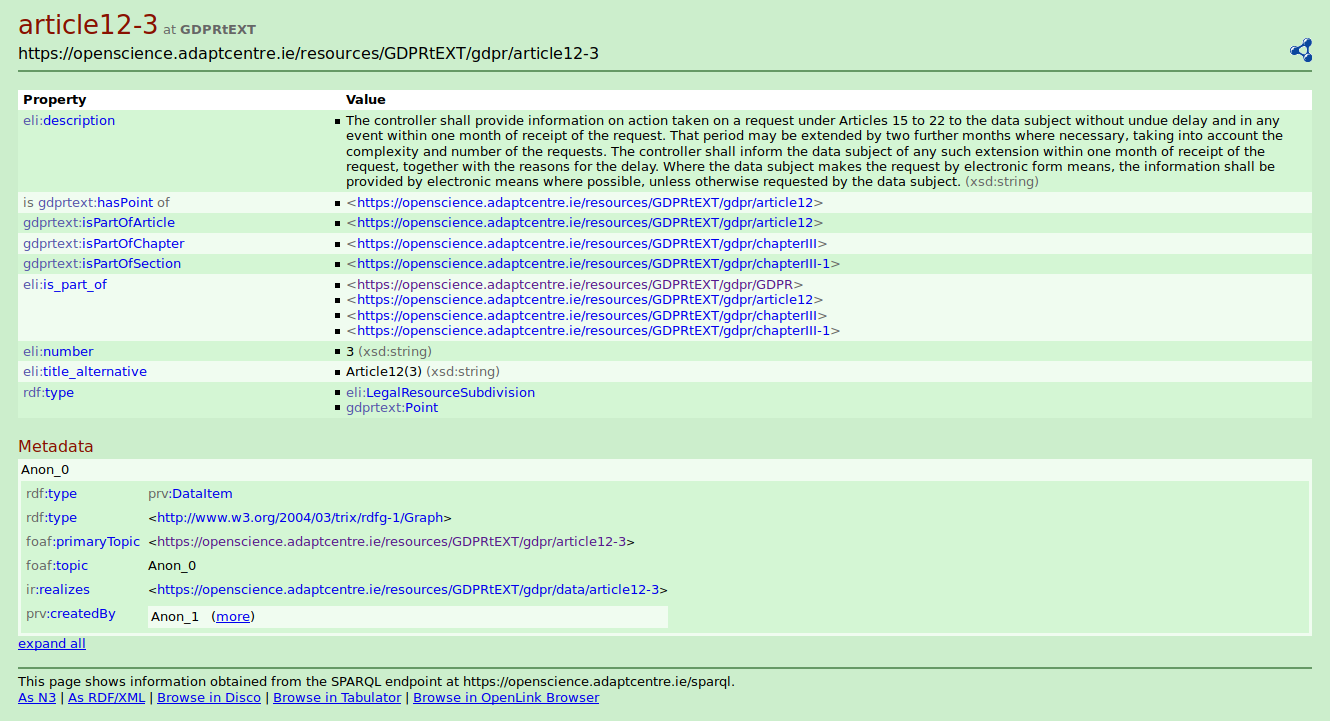
\includegraphics[width=\linewidth]{img/gdprtext-pubby}
    \caption{Article 12(3) in GDPRtEXT as RDF displayed using Pubby \cite{pandit_gdprtext_2018}}
    \label{fig:vocab:gdprtext-pubby}
\end{figure}

\subsection{Resource Description \& Application}
An visual overview of concepts within GDPRtEXT is presented in \autoref{fig:vocab:gdprtext-summary-a} and \autoref{fig:vocab:gdprtext-summary-b}.

\begin{figure}[htbp]
    \centering
    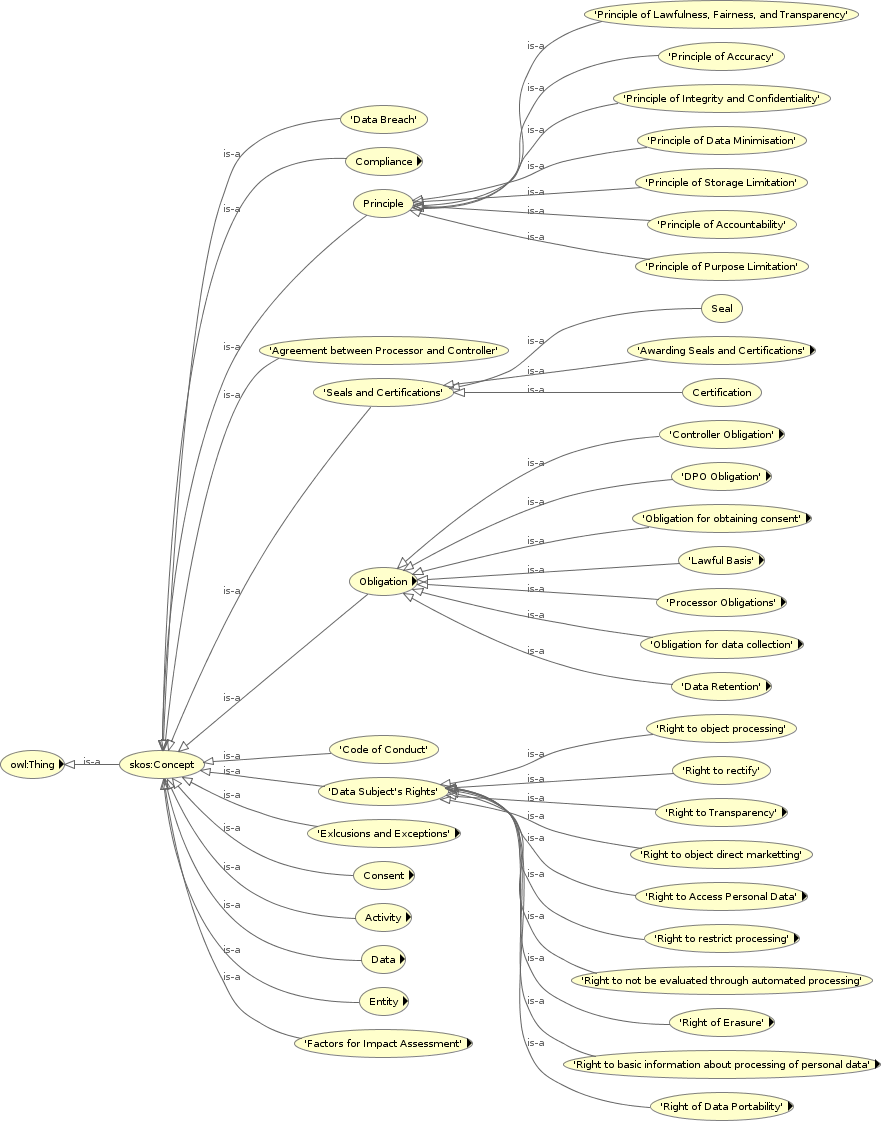
\includegraphics[width=\linewidth]{img/gdprtext-summary-a}
    \caption{Visual overview of concepts in GDPRtEXT - part (a) \cite{pandit_gdprtext_2018}}
    \label{fig:vocab:gdprtext-summary-a}
\end{figure}
\begin{figure}[htbp]
    \centering
    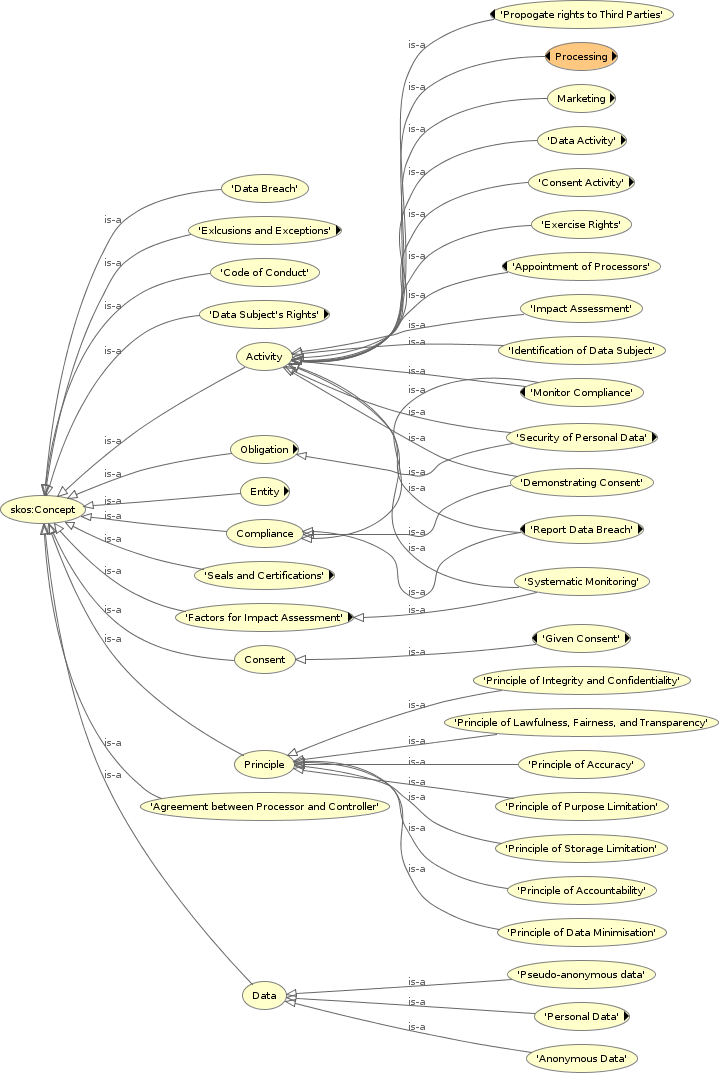
\includegraphics[width=0.75\linewidth]{img/gdprtext-summary-b}
    \caption{Visual overview of concepts in GDPRtEXT - part (b) \cite{pandit_gdprtext_2018}}
    \label{fig:vocab:gdprtext-summary-b}
\end{figure}

\subsubsection{Concepts for description structure of text}
GDPRtEXT extends European Legislation Identifier (ELI) \cite{thomas_european_2019} ontology published by European Publications Office with granular concepts to represent individual clauses within GDPR. 
ELI provides the class \texttt{LegalResource} to indicate a legislative document and its sub-class \texttt{LegalSubResource} to indicate a component or part of that resource. GDPRtEXT extends \texttt{LegalSubResource} with sub-classes \texttt{Chapter}, \texttt{Section}, \texttt{Article}, \texttt{Point} (indicating Paragraph), \texttt{SubPoint} (indicating Sub-Paragraph), \texttt{Recital}, and \texttt{Citation}.
ELI provides properties \texttt{has\_part} and its inverse \texttt{is\_part\_of} to indicate connections between two legal resources, which GDPRtEXT extends using sub-properties to indicate hierarchical relations between chapters, sections, articles, points, and sub-points.

\subsubsection{Concepts about Data}
GDPR mentions different types of data which determine applicable obligations and requirements of compliance. GDPRtEXT provides \texttt{Data} as a top-level concept to indicate abstract term of `data'.
GDPR primarily focuses on personal data as defined in Article 4(1) -  represented in GDPRtEXT as \texttt{PersonalData}, with special categories of personal data defined in Article 9(1) requiring additional obligations for processing and handling being represented by \texttt{SpecialCategoryPersonalData}. Types of special categories mentioned include criminal data, genetic data, health data, and racial data - which are defined as sub-classes in GDPRtEXT.
GDPR also mentions data in context of anonymisation and pseudo-anonymisation processes - represented in GDPRtEXT as \texttt{AnonymousData} and \texttt{PseudoAnonymousData}.

\subsubsection{Concepts about Consent}
The top-level concept of `consent' is represented by \texttt{Consent} in GDPRtEXT with its definitions based in Articles 4(11), 6(1) and Recitals 32, 40. It is sub-classed as \texttt{GivenConsent} - which is a legal basis and therefore is also a sub-class of \texttt{LegalBasis}. \texttt{GivenConsent} is further sub-classed to indicate `valid consent' which carries obligations of ensuring consent is valid and meets requirements of GDPR - and is therefore also defined as sub-class of \texttt{ObligationForObtainingConsent}. Obligations regarding conditions of valid consent are represented by sub-classing the \texttt{ValidConsent} for indicating - freely given, informed, specific, voluntary, and opt-in.

\subsubsection{Concepts about Entities}
\texttt{Entity} represents an `entity' which could be an individual, institution, company, corporation, partnership, or government agency - to name a few. 
It is sub-classed to indicate entities specifically mentioned in GDPR: Data Subject, Controller, Processor, Sub-Processor, Data Protection Officer (DPO), and Data Protection Authority (DPA). Additionally, relevant concepts associated with entities are also defined:  Representative of Controller, Representative of Processor, Certification Body, and Regulatory Authority.

\subsubsection{Concepts about Activities}
`Activity' refers to some process or action mentioned, referred, implied, or defined by requirements of GDPR compliance. To represent these, GDPRtEXT defines activities regarding consent and personal data processing, as well as other activities related to functioning of GDPR - such as reporting data breach and demonstrating consent. The top-level concept `Activity' represents abstraction of all activities. `ConsentActivity' and `DataActivity' represent specialised activities involving consent and personal data respectively.

Consent activities defined within GDPRtEXT consist of obtaining consent and withdrawing consent. Data activities include use, archival, collection, cross-border transfer, erasure, copying, rectifying, sharing, and storage of personal data. In these, the activity associated with usage of personal data is equivalent to its common and synonymous usage with term `processing'. Activities for indicating context of processing include - automated processing,  automated decision making with significant effects, confirming or matching datasets, large scale processing, processing affected or vulnerable individuals, processing sensitive data, processing using untested technologies, and unlawful processing.

GDPRtEXT also provides activities associated with reporting of data breach, which includes obligations and actions such as - report data breach, maintain record of breach, notify data subject of breach, report breach to controller (for processors), and report breach to DPA within 72 hours. Other activities provided are - security of personal data, appointment of processors, demonstrating consent, exercise rights, identification of data subject, impact assessment, marketing, direct marketing, monitor compliance, propagate rights to third parties, and systematic monitoring.

\subsubsection{Concepts about Compliance}
Concepts associated with compliance are provided to indicate actions or terms used in process of maintaining, documenting, evaluating, and demonstrating compliance. The top-level concept \texttt{Compliance} represents an abstract notion of compliance. Other terms derived from this include - Demonstration of Consent, Monitor Compliance, and Report Data Breach.

\subsubsection{Concepts about Principles}
GDPRtEXT represents principles using top-level concept \texttt{Principle}, which is specialised to indicate principles associated with: Accountability; Accuracy; Data Minimisation; Integrity and Confidentiality; Lawfulness, Fairness, and Transparency; Purpose Limitation; and Storage Limitation.

\subsubsection{Concepts about Rights}
To represent rights, GDPRtEXT provides top-level concepts representing each individual right with further concepts associated each right represented as sub-classes. 
The right of data portability is represented by \texttt{RightOfDataPortability} with related concepts regarding: providing copy of personal data, commonly used data format, machine readable format, structured, and supporting reuse.

The right of erasure is represented by \texttt{RightOfErasure} with related concepts provided regarding obligation to erase data when consent is withdrawn, or when data is no longer needed for original purpose. The right to access personal data is represented by concept \texttt{RightToAccessPersonalData} with related concepts for indicating if and where controller is processing data, whether there is automated processing with significant effects on data subject, categories of data being processed, categories of recipients data is shared with, existence of rights, information about processing, source of data, storage period, and ensuring no charges are levied for provision of rights.

\texttt{RightToBasicInformationAboutProcessing} represents right to basic information about processing and is accompanied with its related concept regarding information about third parties. The concept \texttt{RightToRestrictProcessing} represents right to restrict processing, and is accompanied with conditions such as - accuracy is contested, data no longer needed for original purpose, and processing is unlawful. The right to transparency is represented by \texttt{RightToTransparency} with related concepts regarding conditions of concise, easily accessible, intelligible, and transparent. Other represented rights include: right to not be evaluated through automated processing, right to object to direct marketing, right to object to processing, and right of rectification.

\subsubsection{Concepts about Obligations}
GDPRtEXT defines concepts regarding obligations of controllers, processors, DPOs, consent, and compliant processing of personal data based on a legal basis. Obligations of controllers are represented by \texttt{ControllerObligation} with related concepts provided regarding  appointment of processors, accountability, controller responsibility, co-operation with DPA, data protection by design and default, data security, liability of joint controller(s), maintaining records of processing activities, privacy by design, propagate rights to third parties, and reporting data breach.

Rights of processors is represented by \texttt{ProcessorObligaion} with related concepts for appointing sub-processors, assisting in complying with rights, compliance with controller's instructions, co-operating with DPA, data security, imposing confidentiality on personnel, informing controller of conflict with law, maintaining records of processing activities, only acting on documented instructions, propagating rights to third parties, providing controller with information for compliance, reporting data breach to controller, restrictions on cross-border transfers, and to return or destroy personal data at end of term.

The concept \texttt{DPOObligation} represents obligations of a DPO which include the monitoring of compliance represented by \texttt{MonitoringCompliance} . The obligations related to lawful basis for processing are represented by \texttt{LawfulBasisForProcessing} along with related concepts for contract with data subject, exempted by national law, employment law, given consent, historic, statistical, or scientific purposes, legal claims, legal obligation, legitimate interest, made public by data subject, medical or diagnostics use, not for profit organisation, public interest, purpose of new processing, and vital interest.

Obligations regarding valid consent are represented by \texttt{ValidConsent} with related concepts provided to indicate consent should be freely given, informed, specific, voluntary, and opt-in. 
Obligations for obtaining consent are represented by \texttt{ObligationForObtainingConsent} and include concepts for information about third parties, indicating consent can be withdrawn easily, and conditions regarding information provided for obtaining consent such as - it should be clear, providing explanation of processing, should not be from silence or inactivity, should be demonstrable, should be distinguishable from other matters, and that it should produce valid consent.

Obligations for data collection are represented by \texttt{ObligationForDataCollection}, which is accompanied with related concepts for indicating accurate collection, specification of explicit purpose, ensuring legitimate purpose, ensuring it is not further processed than original purpose, and ensuring it is limited to specified purpose.
Obligations for retention of personal data are represented by \texttt{ObligationForRetentionOfPersonalData} and include related concepts about    retention of personal data, ensuring it is adequate for processing, ensuring it is identifiable for required processing, obligation to kept it up to date, ensuring it is limited for processing, obligation to rectify inaccuracies, and ensuring it is relevant for processing. 
The concept \texttt{ObligationForSecurityOfPersonalData} represents obligations regarding security of personal data with related concepts provided regarding accidental loss, damage, destruction, and unlawful processing.

\subsubsection{Concepts about Seals and Certifications}
GDPRtEXT provides concepts of \texttt{Seal} and \texttt{Certification} for representing seals and certifications as provided by GDPR to assist with maintenance and demonstration of compliance.
The conditions of these are represented by \texttt{ConditionsForSealsAndCertifications}, which is further expanded to represent conditions for seal/certification such as having a maximum validity of 3 years and having a voluntary system of accreditation. 

\subsubsection{Example Use-Case: Compliance Reporting}
This example use-case, taken from documentation of GDPRtEXT \cite{pandit_gdprtext_2018}, shows how references to GDPR can aid in creation of reports which document information regarding compliance. 

Consider a system for creation of compliance reports that stores information related to obligations it addresses from GDPR. It uses the EARL\footnote{\url{https://www.w3.org/TR/EARL10-Schema/}} vocabulary for expressing results of conformance checks within the report. GDPRtEXT is used to link resources in EARL reports with articles and points within GDPR and to express and define concepts related to compliance in a suitable and comprehensible manner. Through this, information about compliance checks is linked and associated with specific articles of GDPR.

EARL provides a standardised vocabulary to describe specific resources and relationships that are relevant to test reporting. The core construct of EARL is an \texttt{Assertion}, which describes context and outcome of an individual test execution. It uses following concepts (copied verbatim from EARL specification):

\begin{itemize}
    \item \texttt{Assertor} - This can include information about who or what ran the test. For example human evaluators, automated accessibility checkers, or combinations of these.
    \item \texttt{Test Subject} - This can include web content (such as web pages, videos, applets, etc.), software (such as authoring tools, user agents, etc.), or other things being tested.
    \item \texttt{Test Criterion} - What are we evaluating test subject against? This could be a specification, a set of guidelines, a test from a test suite, or some other testable statement.
    \item \texttt{Test Result} - What was the outcome of test? A test result could also include contextual information such as error messages or relevant locations.
\end{itemize}

Taking the example of Right to Data Portability, the EARL report in \autoref{earl} represents compliance checks for conditions associated with linked articles in GDPR (Article 20). The compliance system has a module \texttt{\_system\_dataportability} that checks software that handles provision of copy of personal data \texttt{\_org\_dataportability} through test case \texttt{\_test\_provide\_data\_copy} and generates a report showing the test has passed through \texttt{\_result\_pass}.


\begin{listing}
\begin{minted}{turtle}
@prefix earl: http://www.w3.org/ns/earl# .
@prefix dct:  http://purl.org/dc/terms/ .
@prefix gdprtext: http://purl.org/adaptcentre/resources/GDPRtEXT# .

_org_dataportability
    a    earl:TestSubject, earl:Software ;
    dct:description "System that handles data portability requests"@en ;
    dct:title "Data Portability Handler"@en .

_system_dataportability
    a    earl:Assertor ;
    dct:description "Module checking data portability obligations"@en ;
    dct:hasVersion "1.4" ;
    dct:title "DataPortability Module"@en ;
    earl:asserts { 
      _org_dataportability _result_pass _test_provide_data_copy } .

_result_pass
    a    earl:ResultProperty ;
    earl:date "2018-01-01" ;
    earl:validity earl:Pass ;
    earl:confidence earl:High .

_test_provide_data_copy
    a    earl:TestCase ;
    earl:testMode earl:automatic ;
    dct:title "Test provision of data copy"@en ;
    dct:description "Tests whether system provides a copy 
      of personal data on exercising right to data portability"@en ;
    dct:subject gdprtext:article20 .
\end{minted}
\caption{Use of GDPRtEXT to link tests with GDPR Articles in EARL report}
\label{earl}
\end{listing}

To gather related resources together, a SPARQL query (simplified) would focus on link between \texttt{TestCase} and its result using \texttt{earl:validity}, as shown in \autoref{code:voc:gdprtext-sparql}.
These tests can be further combined into test suites to group compliance checks related to each article or a particular concept and structure  documentation around this form of logical grouping of concepts.
In this manner, use of GDPRtEXT to link tests and results with documentation enables automation of information retrieval and management.
A similar use-case of GDPRtEXT in linking constraints and their outcomes with GDPR is demonstrated in \autoref{chapter:testing}.

\begin{listing}
\begin{minted}{sparql}
SELECT ?gdpr ?result ?confidence ?mode WHERE {
    ?assertor a earl:Assertor .
    ?assertor earl:asserts ?assertion .

    ?testcase rdf:predicate ?assertion .
    ?testcase a earl:TestCase .
    ?testcase dct:subject ?gdpr .
    ?testcase ear:testMode ?mode .

    ?testresult rdf:object ?assertion .
    ?testresult a earl:ResultProperty .
    ?testresult earl:validity ?result .
    ?testresult earl:confidence ?confidence .
}

| gdpr          | result     | confidence     | mode          |
---------------------------------------------------------------
| article16     | pass       | low            | automatic     |
| article17     | pass       | high           | automatic     |
| article18     | fail       | high           | manual        |
| article19     | pass       | high           | automatic     |
\end{minted}
\caption{SPARQL query and results showing retrieved GDPR test results by article}
\label{code:voc:gdprtext-sparql}
\end{listing}

\subsubsection{Example Use-Case: Mapping between DPD and GDPR obligations}
The second application of GDPRtEXT, taken from its publication \cite{pandit_gdprtext_2018}, demonstrates linking of obligations between GDPR and its predecessor - Data Protection Directive (DPD. Given that DPD was adopted in 1995, and was superseded by GDPR in 2016, there are a large number of solutions and approaches regarding compliance with DPD that already exist and are used in practice. By linking obligations between DPD and GDPR it is possible to investigate reuse of these existing solutions for GDPR compliance. To that end, a mapping from DPD obligations to GDPR obligations containing annotations that describe nature of changes is constructed by linking articles of DPD and GDPR.

To model annotations as a RDF resource, a linked data version of DPD was created similar to GDPRtEXT by assigning URIs for every clause in legislation. This enabled referring to each individual clause in DPD and linking it with relevant clauses in GDPR. 
The annotations (available online\footnote{\url{https://openscience.adaptcentre.ie/projects/GDPRtEXT/dpd_mapping.html}}) consist of references from a clause in DPD to its corresponding clause in GDPR with an expression of change between the two. The nature of change is represented by values: same - indicating no change; reduced - indicating reduction of obligation; slightly changed - indicating minor change; completely changed - indicating major change; and extended - indicating addition of obligations.

Its example demonstration consisted of using XACML\footnote{\url{https://www.oasis-open.org/committees/tc_home.php?wg_abbrev=xacml}} rules for controlling access to data and modelled after DPD obligations.
For each link between DPD and GDPR obligations, a record was created indicating whether the corresponding XACML rules for DPD compliance needed to be changed to be applicable for GDPR. The notation \texttt{N/A} was used to denote cases where no XACML rules existed for a particular DPD obligation and where corresponding obligations in GDPR had changed or had additional requirements. 
\begin{listing}[htbp]
\begin{minted}{turtle}
@prefix gdpr: https://w3id.org/GDPRtEXT/gdpr# .
@prefix dpd: https://w3id.org/GDPRtEXT/dpd# .
@prefix rdfs: http://www.w3.org/2000/01/rdf-schema# .

dpd:mappingrule6
    a dpd:DPDToGDPR_Annotation ;
    dpd:hasChange dpd:ChangeExtended ;
    dpd:hasXACMLChange dpd:XACMLNoChange ;
    dpd:resourceInDPD dpd:Article7 - a ;
    dpd:resourceInGDPR gdpr:Article6-1-a ;
    rdfs:comment "added consent given to ..." .
\end{minted}
\caption{Example annotation of associating existing DPD compliance XACML rules with requirements of GDPR}
\label{code:voc:gdprtext-xacml}
\end{listing}
% The value \texttt{No} was used to indicate no changes in the GDPR obligation compared to the DPD obligation, so that the existing XACML rule would be sufficient to meet GDPR requirements. Similarly \texttt{Yes} was used to indicate a change required in the XACML rule to handle the obligation.

The class \texttt{DPDToGDPR\_Annotation} represents annotations between DPD and GDPR, with an example instance depicted in \autoref{code:voc:gdprtext-xacml}. The property \texttt{resourceInDPD} is used to refer to a specific clause within DPD using its IRI. Similarly, the property \texttt{resourceInGDPR} is used to refer to a corresponding clause in GDPR. The nature of change is defined using property \texttt{hasChange} whose value is an instance of class \texttt{ChangeInObligation}, with instances defined for \textit{Extended, Same, Reduced, CompletelyChanged}, and \textit{SlightlyChanged}. Similarly, a change in XACML rules is defined using class \texttt{ChangeInXACMLRule} with instances \textit{Yes, No}, and \textit{N/A}.

\subsection{Evaluation}\label{sec:voc:gdprtext:evaluation}
In terms of ontology assessment, the methodology outlined in \autoref{sec:voc:methodology} provides criterion for evaluation of ontology quality and documentation. GDPRtEXT fulfils these based on using OOPS! tool\footnote{OOPS! results published with ontology documentation. The results can also be independently obtained using the OOPS! online service.} to identify and rectify bad design patterns and by following best practices and community guidelines for ontology documentation.
GDPRtEXT and the work described in this section was published \cite{pandit_gdprtext_2018} at Extended Semantic Web Conference (ESWC) - Resource Track. The publication described creation of resource, summarised its contents, and described mapping of DPD obligations with GDPR using a linked data approach and XACML to denote which obligations from DPD could be re-used towards GDPR compliance. 
ESWC is a premier and top-tier conference within semantic web domain, and has a rigorous review process with an open review policy.
The acceptance of GDPRtEXT in this venue demonstrates its value as a semantic web resource.

To date, the publication has received 19 citations from peer-reviewed publications (excluding self-citations) on Google Scholar\footnote{\url{https://scholar.google.com/scholar?cites=2776106745007214232}}.
In addition to these, a 5 star rating given to GDPRtEXT as a dataset in Irish open data portal indicates its adherence to linked data principles.
% The publications associated with PrOnto \cite{palmirani_pronto_2018,palmirani_pronto_2018-1} cite GDPRtEXT as a resource of GDPR concepts and comment on  modelling of the norms and the legal axioms - which are not within the scope of GDPRtEXT or this thesis. It also mentions the lack of FRBR
% \footnote{Functional Requirements for Bibliographic Records (FRBR) is a conceptual entity–relationship model which allows expressing legal text as an abstract document with expressions in different languages and manifestations in different representations. It was adopted for use in ELI in the legislation passed on 6 November 2017 (OJ C 441, 22.12.2017, p. 8–12 \url{https://eur-lex.europa.eu/legal-content/EN/TXT/?uri=CELEX:52017XG1222(02)}).}
% information for managing versioning of the legal text over the time.
% However, it must be noted that since the ELI ontology itself uses FRBR and that GDPRtEXT extends ELI, it is capable of supporting the FRBR concepts as well - but does not provide them since the aim of the work is to enable granular references to its clauses rather than a provision of its text in multiple languages and representations. 
A survey of legal approaches within state of the art \cite{leone_taking_2019} undertaken by MIREL project analysed GDPRtEXT amongst other legal ontologies and found that GDPRtEXT is singular in its use of ELI and provision of GDPR as a glossary of concepts - a finding shared with the analyses of SotA in \autoref{sec:sota:analysis}.

\subsubsection{Fulfilment of Competency Questions}
The assessment of GDPRtEXT consists of evaluating the extent to which it answers competency questions outlined in \autoref{sec:voc:gdprtext-engineering}.
For this, \autoref{table:gdprtext:eval-cq} shows concepts and relationships of GDPRtEXT relevant towards answering competency questions.
\begin{center}
    \footnotesize
\begin{tabularx}{\textwidth}{|l|X|}
\caption{Concepts in GDPRtEXT for answering competency questions} \label{table:gdprtext:eval-cq} \\
\toprule
\textbf{CQ} & \textbf{Concepts/Relationships} \\
\midrule
\endfirsthead

\caption*{Concepts in GDPRtEXT for answering competency questions (cont'd)} \\
\toprule
\textbf{CQ} & \textbf{Concepts/Relationships} \\
\midrule
\endhead

\midrule
\multicolumn{2}{r@{}}{\footnotesize (Cont'd on following page)}\\
\endfoot

\endlastfoot

% & \textbf{Concepts associated with structure of GDPR} \\ \hline
\textit{CQ1-7} & \textit{Recital, Chapter, Section, Article, Point, SubPoint, Reference, Citation} \\ \hline
% \textit{CQ2} & \textit{Chapter} \\ \hline
% \textit{CQ3} & \textit{Section} \\ \hline
% \textit{CQ4} & \textit{Article} \\ \hline
% \textit{CQ5} & \textit{Point} \\ \hline
% \textit{CQ6} & \textit{SubPoint} \\ \hline
% \textit{CQ7} & \textit{Reference}, \textit{Citation} \\ \hline
\textit{CQ8} & \textit{isPartOfChapter} \\ \hline
\textit{CQ9,11} & \textit{rdfs:isDefinedBy [Article, Point, SubPoint]} \\ \hline
\textit{CQ10} & \textit{:\_ hasPart/isPartOf :\_} \\ \hline
% \textit{CQ11} & \textit{Accountability} \\ \hline
\textit{CQ12} & \textit{:GivenConsent rdfs:seeAlso [Article, Point, SubPoint]} \\ \hline
% \textit{CQ13} & \textit{GivenConsent} \\ \hline
\textit{CQ13,14} & \textit{GivenConsent/Compliance :involves [Article, Point, SubPoint]} \\ \hline

% & \textbf{Concepts associated with GDPR compliance} \\ \hline
\textit{CQ15} & \textit{Data}, \textit{PersonalData}, \textit{SensitivePersonalData}, \textit{CriminalData}, \textit{GeneticData}, \textit{HealthData}, \textit{RacialData}, \textit{AnonymousData}, \textit{PseudoAnonymousData} \\ \hline
\textit{CQ16} & \textit{Consent}, \textit{GivenConsent}, \textit{WithdrawnConsent} \\ \hline
\textit{CQ17} & \textit{Entity}, \textit{DataSubject}, \textit{Controller}, \textit{JointController}, \textit{Processor}, \textit{SubProcessor}, \textit{DPO}, \textit{DPA}, \textit{ControllerRepresentative}, \textit{ProcessorRepresentative}, \textit{CertificationBody}, \textit{RegulatoryAuthority} \\ \hline
\textit{CQ18,19} & \textit{DataActivity, ConsentActivity} \\ \hline
% \textit{CQ19} & \textit{ConsentActivity} \\ \hline
\textit{CQ20} & \textit{Processing}, \textit{AutomatedProcessing}, \textit{AutomatedDecisionMakingWithSignificantEffect}, \textit{ConfirmingOrMatchingDatasets}, \textit{LargeScaleProcessing}, \textit{ProcessingAffectedOrVulnerableIndividuals}, \textit{ProcessingSensitiveData}, \textit{ProcessingUsingUntestedTechnologies}, \textit{Unlawful} \textit{Processing} \\ \hline
\textit{CQ21} & \textit{ReportDataBreach}, \textit{MaintainRecordOfBreach},  \textit{NotifyDataSubjectOfBreach}, \textit{ReportBreachToController}, \textit{ReportBreachToDPAWithin72Hours} \\ \hline
\textit{CQ22} & \textit{Compliance}, \textit{Demonstration}, \textit{ConsentMonitor}, \textit{Compliance}, \textit{ReportDataBreach}  \\ \hline
\textit{CQ23} & \textit{Principle}, \textit{Accountability}, \textit{Accuracy}, \textit{DataMinimisation}, \textit{IntegrityAndConfidentiality}, \textit{LawfulnessFairnessAndTransparency}, \textit{PurposeLimitation}, \textit{StorageLimitation}  \\ \hline
\textit{CQ24} & \textit{Rights}, \textit{RightOfDataPortability}, \textit{RightOfErasure}, \textit{RightToAccessPersonalData}, \textit{RightToTransparency}, \textit{RightToBasicInformationAboutProcessing}, \textit{RightToNotBeEvaluatedThroughAutomatedProcessing}, \textit{RightToObjectForDirectMarketting}, \textit{RightToObjectToProcessing}, \textit{RightToRectify}, \textit{RightToRestrictProcessing} \\ \hline
\textit{CQ25} & \textit{RightOfDataPortability}, \textit{ProvideCopyOfPersonalData}, \textit{ShouldBeCommonlyUsedFormat}, \textit{ShouldBeMachineReadable}, \textit{ShouldBeStructured}, \textit{ShouldSupportReuse}  \\ \hline
\textit{CQ26} & \textit{RightToBasicInformationAboutProcessing}, \textit{InformationAboutThirdParties}  \\ \hline
% \textit{CQ27} & \textit{Obligation} \\ \hline
\textit{CQ27,28} & \textit{Obligation, ControllerObligation}, \textit{AppointmentOfProcessors}, \textit{Accountability}, \textit{ControllerResponsibility}, \textit{CooperateWithDPA}, \textit{DataProtectionByDesignAndDefault}, \textit{DataSecurityLiabilityOfJointControllers}, \textit{MaintainRecordsOfProcessingActivities}, \textit{PrivacyByDesign}, \textit{PropogateRightsToThirdParties}, \textit{ReportDataBreach} \\ \hline
\textit{CQ29} & \textit{ProcessorObligation}, \textit{AppointingSubprocessors}, \textit{AssistInComplyingWithRights}, \textit{ComplianceWithControllersInstructions}, \textit{CooperateWithDpa}, \textit{DataSecurity}, \textit{ImposeConfidentialityOnPersonnel}, \textit{InformControllerOfConflictWithLaw}, \textit{MaintainRecordsOfProcessingActivities}, \textit{OnlyActOnDocumentedInstructions}, \textit{PropogateRightsToThirdParties}, \textit{ProvideControllerWithInformationForCompliance}, \textit{ReportDataBreachToController}, \textit{RestrictionsOnCross}-\textit{borderTransfers}, \textit{ReturnOrDestroyPersonalDataAtEndTerm} \\ \hline
\textit{CQ30} & \textit{DPOObligation}, \textit{MonitorCompliance} \\ \hline
\textit{CQ31} & \textit{LawfulBasisForProcessing}, \textit{ContractWithDataSubject}, \textit{ExemptedByNationalLaw}, \textit{EmploymentLaw}, \textit{GivenConsent}, \textit{HistoricStatisticalOrScientificPurposes}, \textit{LegalClaims}, \textit{LegalObligation}, \textit{LegitimateInterest}, \textit{MadePublicByDataSubject}, \textit{MedicalDiagnosticOrTreatement}, \textit{NotForProfitOrg}, \textit{PublicInterest}, \textit{PurposeOfNewProcessing}, \textit{VitalInterest} \\ \hline
\textit{CQ32} & \textit{ValidConsent}, \textit{FreelyGivenConsentObligation}, \textit{InformedConsentObligation}, \textit{SpecificConsentObligation}, \textit{VoluntaryOptInConsentObligation}  \\ \hline
\textit{CQ33} & \textit{ObligationForDataCollection}, \textit{AccurateCollection}, \textit{ExplicitPurpose}, \textit{LegitimatePurpose}, \textit{NotFurtherProcessedThanOriginalPurpose}, \textit{SpecifiedPurpose} \\ \hline
\textit{CQ34} & \textit{InformationAboutThirdParties}, \textit{ConsentCanBeWithdrawnEasily}, \textit{ClearExplanatinOfProcessing}, \textit{NotFromSilenceOrInactivity}, \textit{Demonstrable}, \textit{DistinguishableFromOtherMatters}, \textit{ValidConsent} \\ \hline
\textit{CQ35} & \textit{RetentionOfPersonalData}, \textit{AdequateForProcessing}, \textit{IdentifiableForRequiredProcessing}, \textit{KeptUpToDate}, \textit{LimitedForProcessing}, \textit{RectifyInaccuracies}, \textit{RelevantForProcessing} \\ \hline
\textit{CQ36} & \textit{SecurityofPersonalData}, \textit{AccidentalLoss}, \textit{Damage}, \textit{Destruction}, \textit{UnlawfulProcessing} \\ \hline
\textit{CQ37} & \textit{Seal}, \textit{Certification} \\
\bottomrule
\end{tabularx}
\end{center}
The table demonstrates that GDPRtEXT provides concepts to answer all  competency questions. GDPRtEXT thus meets requirements of representing and linking information with text and concepts of GDPR in a granular manner and fulfils $RO3(a)$.

\subsubsection{Comparison with SotA}
The SotA in representing text of GDPR in machine-readable formats presented in \autoref{sota:analysis:representation} compared three approaches: ELI \cite{thomas_european_2019}, Agarwal et al \cite{agarwal_legislative_2018}, and PrOnto \cite{palmirani_pronto_2018,palmirani_pronto_2018-1}.
Their comparison and analysis, summarised in \autoref{table:sota:analysis:GDPR}, depicts relevance of each approach in representing the GDPR as a glossary of concepts, providing a permanent identifier for resources, modelling of GDPR's text, and whether resources are open and accessible.
The conclusion drawn from these is the lack of an approach fulfilling all criteria along with a lack of open and reusable resources concerning GDPR. 
The additional resource of ELI+ mentioned in analysis shows intention of EU Publications Office to remedy this gap through an update to the ELI ontology at some time in future.

A comparison of GDPRtEXT with these approaches, depicted in \autoref{table:gdprtext:sota}, shows that GDPRtEXT provides a glossary of concepts, uses permanent identifiers, provides linked data version of text of GDPR, and is available under an open and permissive license (CC-BY-4.0).
This matches the intended contributions of ELI+ (update to ELI) planned by EU Publications Office, and therefore enables GDPRtEXT to fill this gap in this time.
\begin{center}
    \footnotesize
\begin{tabularx}{\textwidth}{|l|>{\columncolor[gray]{0.9}}l|l|l|l|l|}
    \caption{Comparison of GDPRtEXT with SotA}\label{table:gdprtext:sota} \\
\toprule
Work & \textbf{GDPRtEXT} & ELI & ELI+ & Agarwal et al & PrOnto \\
\midrule
\endhead

Vocabulary & ELI & OWL2 & OWL2 & RDFS & Akoma Ntoso \\ \hline
Granularity & Sub-Paragraph & Legislation & Sub-Paragraph & Paragraph & Sub-Paragraph \\ \hline
Glossary & \cmark & \xmark & \cmark & \xmark & \xmark \\ \hline
PID & \cmark & \cmark & \cmark & \xmark & \xmark \\ \hline
OA & \cmark & \cmark & \cmark & \xmark & \xmark \\ \hline
GDPR text & \cmark & \xmark & \cmark & \xmark & \cmark \\
\bottomrule
\end{tabularx}
\end{center}

A survey of legal ontologies by Leone et al. \cite{leone_taking_2019} includes GDPRtEXT as an ontology relevant for data protection. The survey also includes ELI and PrOnto within the scope of data protection ontologies - which provides external comparison between these and GDPRtEXT. The survey outlines the role of GDPRtEXT in acting as a glossary of concepts rather than a prescriptive set of norms and rules for specification of compliance - such as made available through PrOnto. In this role, GDPRtEXT is novel within state of the art given a lack of other similar resources.

Based on this, GDPRtEXT is argued to provide novel contribution to state of the art and addresses gaps associated with representation of concepts and GDPR text at a granular level, and whose open availability enables usage and adoption.

\subsection*{Summary}
The GDPRtEXT resource represents the first major contribution of this thesis. It provides a linked data version of text of GDPR and a glossary of its concepts, fulfils research objective $RO3(a)$, and assists with research objective $RO5(b)$ - as outlined in \autoref{sec:intro:RQ}. It enables representing each article or point within GDPR as a unique resource through IRIs defined using RDF and semantic web.
GDPRtEXT thus enables machine-readable links to be established between information and clauses of GDPR as well as concepts pertaining to its compliance.

The use of GDPRtEXT makes it possible to create approaches that automate generation and querying of information associated with GDPR - such as for compliance, management of business processes, or generation of privacy policies. The compatibility provided through extension of ELI ontology ensures alignment with official documents produced by European Publications Office.
Finally, GDPRtEXT fills an important gap in the state of the art regarding machine-readable approaches for linking information with legal text.
GDPRtEXT has been released as an open resource, has been published in Zenodo and Datahub, and has been incorporated into Ireland’s open data portal as a 5-star linked open dataset.

% GDPRov
\section{GDPRov - Ontology for GDPR activities associated with Personal Data and Consent}\label{sec:voc:GDPRov}
This section describes the GDPRov ontology for representing activities in ex-ante and ex-post phases associated with processing of personal data and consent for GDPR compliance. GDPRov stands for GDPR Provenance - a reference to the requirement of maintaining provenance information of processes in both ex-ante and ex-post phases for demonstrating GDPR compliance. This section presents motivation, overview, dissemination, and evaluation of GDPRov ontology. It also presents comparisons with relevant approaches in state of the art. 

The ontology satisfies the research objectives $RO3(b)$ presented in \autoref{sec:intro:RQ}.
It uses the compliance questions presented in \autoref{sec:info:compliance-questions} as competency questions to identify requirements and for evaluation.
GDPRtEXT is used to define and associate the source of concepts within the text of GDPR.
An earlier version (v0.4) of GDPRov was described in a peer-reviewed publication \cite{pandit_modelling_2017}.
Subsequent revisions included addition of new concepts associated with real-world implementation and interpretation of GDPR compliance requirements (see \autoref{sec:testing:sparql}) and for representing information about consent mechanisms on the internet (see \autoref{sec:testing:shacl}).
The latest version of GDPRov (v0.7) is available online\footnote{\url{http://w3id.org/GDPRov}} with its documentation and code repository\footnote{\url{https://github.com/coolharsh55/GDPRov}}.

\subsection{Identification of requirements from competency questions}\label{sec:gdprov:cq}
The compliance questions presented in \autoref{sec:info:compliance-questions} were selected based on relevance to information regarding activities and provided competency questions for deriving concepts and relationships regarding processes associated with personal data and consent based on GDPR compliance requirements. 
These concepts and relationships were collected, combined, and analysed to ensure their cohesion as an ontology and evaluated using compliance questions to ensure they satisfied requirements regarding GDPR compliance and documentation of associated processes.
In this, ex-ante and ex-post representation provide repetition of some information as most processes have counterparts in both phases. The linking of information between phases enables them to be documented in a manner so as to demonstrate prior planning of processes to ensure compliance and later their execution which also needs to be documented for compliance.
Therefore, while GDPR requirements and compliance questions do no explicitly mention or refer to ex-ante and ex-post phases for each activity, GDPRov implicitly considers each activity to have representations in both phases.

The sub-sections below present concepts to answer competency questions derived from compliance questions. 
This is followed by an analysis of discovered concepts in ex-ante and ex-post phases.
The analysis is used to derive requirements for construction of GDPRov ontology, and is presented to describe motivations for the ontology design and implementation.

\subsubsection{Actors and Agents involved in activities}
\begin{itemize} 
    \item \texttt{CMQ2} - Provides concept of \textit{Controller} as an agent controlling processes and its representative \textit{Data Protection Officer (DPO)}.
    \item \texttt{CMQ17} - Describes \textit{Processor} as an executor of processes and its representative \textit{DPO}. In this relationship, \textit{Controller} provides processes to be executed as instructions to \textit{Processor} through a \textit{Data Processing Agreement (DPA)}.
    \item \texttt{CMQ35} - Describes \textit{Data Subject} as an agent who is associated with provision of personal data, consent, and who is related to exercising of rights.
\end{itemize}

\subsubsection{Details of processing}
\begin{itemize}
    \item \texttt{CMQ3} and \texttt{CMQ37} provide concept of \textit{Purpose} which describes purpose of personal data processing. Each purpose can incorporate multiple processing operations, and each processing operation taking place can be associated with multiple purposes.
    \item \texttt{CMQ4} describe necessity to specify data subject categories whose personal data is being processed.
    \item \texttt{CMQ36} describes personal data, while \texttt{CMQ5} describes categories of personal data being processed. \texttt{CMQ34} specifies special categories of personal data as a sub-category of personal data that needs to be explicitly stated as being processed.
    \item \texttt{CMQ38} defines processing of personal data as defined by Article 4-2 of GDPR. The GDPR definition of processing provides types of operations as specified by ``\textit{any operation or set of operations which is performed on personal data or on sets of personal data, whether or not by automated means, such as collection, recording, organisation, structuring, storage, adaptation or alteration, retrieval, consultation, use, disclosure by transmission, dissemination or otherwise making available, alignment or combination, restriction, erasure or destruction;}''.
    \item \texttt{CMQ6} defines sharing of data as a type of processing. Additional information associated with sharing of data is provided by - \texttt{CMQ7} and \texttt{CMQ20} for categories of recipients; \texttt{CMQ8},\texttt{CMQ21} for identifies of recipients, \texttt{CMQ9} and \texttt{CMQ22} for location where data is being sharing to; \texttt{CMQ10} and \texttt{CMQ23} for safeguards associated with data transfer; \texttt{CMQ15} and \texttt{CMQ25} for purposes of sharing - which is the same concept as purpose of processing except applied for sharing of personal data.
    \item \texttt{CMQ11} defines data storage, with additional concepts provided by \texttt{CMQ12} for existence of time limits or conditions for erasure and \texttt{CMQ13} for specification of time limits or conditions for erasure for categories of data.
    \item \texttt{CMQ26} defines legal basis for justifying processing of personal data, and \texttt{CMQ27} specifies legal basis associated with a particular purpose. Each purpose can have one or more legal basis associated with it.
\end{itemize}

\subsubsection{Life-cycle of data}
\begin{itemize}
    \item \texttt{CMQ28} and \texttt{CMQ30} describe source of personal data which in turn implies an activity that collects data and specifies actors or agents as source of data.
    \item \texttt{CMQ29} specifically refers to personal data collected from data subject.
\end{itemize}

\subsubsection{Anonymisation}
\begin{itemize}
    \item \texttt{CMQ31} specifies anonymisation of personal data with \texttt{CMQ32} inquiring about different `levels' of anonymisation which affect the application of obligations and requirements of compliance. 
    \item Levels of anonymisation are specified based on their relevance to investigation of compliance, and are defined as data which is: completely anonymised, pseudo-anonymised, not anonymised. In this, data that is pseudo-anonymised can be considered and used as anonymous data when an organisation does not have additional information to de-anonymise it. 
    \item Processing activities associated with anonymisation and de-anonymisation of personal data are defined to produce anonymised data.
\end{itemize}

\subsubsection{Activities associated with Consent}
\begin{itemize}
    \item Regarding consent, \texttt{CMQ48} inquires about activities associated with provision and collection of consent. This includes information about how consent is requested and collected, used within processes as a legal basis, and is archived for future demonstration of compliance.
    \item \texttt{CMQ49} and \texttt{CMQ50} inquire about artefacts associated with collection of consent for determination of consent validity under GDPR, which requires investigation of how choices for consent were offered. This also includes forms through which consent is provided or collected from data subjects. Artefacts such as forms or dialogues are associated with processes where consent choices are offered or requested and whose result is collection of consent or given consent.
\end{itemize}

\subsubsection{Provision of Rights}
\begin{itemize}
    \item The rights associated with GDPR need processes to internally (in perspective of an organisation) handle their execution as well as for interactions with data subjects. Therefore, such processes need to be defined and documented for compliance purposes.
    \item For right to be informed, \texttt{CMQ88 - CMQ105} provide  competency questions regarding how the right is provided and how it is executed or implemented.
    \item This includes activities associated with provision of information to data subject, artefacts associated with information provision, inclusion of details such as controller and DPO, purposes, processing, legal basis, and personal data categories.
    \item It also includes information about sources of personal data (where not obtained directly from data subject), and whether legal basis used is legitimate interest.
    \item Regarding data sharing, information to be specified includes categories of recipients and their location.
    \item Right to be informed also includes provision of information regarding existence and application of rights.
    \item Information associated with right to be informed is common to other information documented in due course of processing of personal data, and therefore does not require a separate notation or representation of this information in order to execute the right. Existing information or concepts for representation of processing activities can be reused for specifying required information. However, activities associated with executing rights need to be defined to demonstrate existence of processes for handling rights.
\end{itemize}

\subsubsection{Compliance procedures such as Reporting of Data Breach}
\begin{itemize}
    \item Reporting of data breach requires information about data breach to be maintained as specified by \texttt{CMQ106 - CMQ120}.
    \item This includes information about the data breach consisting of: timestamp of when breach occurred (\texttt{CMQ106}), timestamp of when controller became aware of it (\texttt{CMQ107}), timestamp and method of it being notified to supervisory authority (\texttt{CMQ108}).
    \item Information about contents of breach include information about its affected personal data and categories of data subject (\texttt{CMQ112}).
    \item Information also needs to be provided to supervisory authorities and in some cases to data subjects based on extent of breach (\texttt{CMQ113}). It therefore requires prior planning of processes for handling data breaches and sending information to data subjects along with any remedial measures (\texttt{CMQ116}).
\end{itemize}

\subsubsection{Specifying requirements for ex-ante and ex-post phases}
Process logs are a convenient and demonstrable form of information to store and document compliant processing of personal data. By verifying logs, it is possible to document, evaluate, and demonstrate that executed processes were compliant with requirements of GDPR. This constitutes as ex-post phase of compliance and consists of evaluating information after processing has been carried out. It also fulfils Article 30 of GDPR concerning processing records to be maintained. Along with ex-post records, it is also essential to demonstrate that executed processes were based on a preconceived plan or template that was ensured to be compliant before execution. Storing such plans is essential to demonstrate prior planning and maintenance of a compliant processing system. This constitutes as ex-ante phase of compliance, and consists of evaluating compliance on plans of processing yet to be carried out. This is necessary for Article 35 of GDPR concerning carrying out a DPIA.

Associating executed processes with their plans allows demonstration of compliance throughout the life-cycle of processes, i.e. from planning of processes to their eventual execution. It also enables documenting changes in plans and their effects on execution of processes - i.e. demonstrating that when a plan changes it also brings about corresponding changes in executed processes. In context of GDPR compliance, requirements of compliance require documentation, maintenance, and demonstration of processes across both ex-ante (planning) and ex-post (execution) phases. Ex-ante plans of processes are described as an organisational measure and their compliance is associated with ensuring processes meet legal requirements before they are actually carried out. In some instances, such as for a Data Protection Impact Assessment (DPIA), existence of ex-ante information about processes is essential in evaluation of compliance.

While compliance questions provide a basis for identifying information to be modelled, requirements of expressing this information in ex-ante and ex-post phase require specification of their intended usage in planning and processing stages respectively which further determines whether compliance evaluation consists of verification of a plan or analysis of processing logs. 
The argument and motivation for representing processes in ex-ante and ex-post phases represents a design decision based on separating representation of information across phases of compliance rather than being a compliance requirement itself.
Approaches within state of the art that also follow a similar representation of ex-ante and ex-post information include SPECIAL (\autoref{sec:sota:SPECIAL}) which uses PROV-O to log information in both phases, and MIREL (\autoref{sec:sota:MIREL}) which uses a workflow model to represent a plan and its executions.

Information requirements for modelling information about activities is summarised through following points:
\begin{enumerate}
    \item Represent process in ex-post phase as a log or record.
    \item Represent process in ex-ante phase as plan or template.
    \item Link ex-ante plan with its instantiations or executions in ex-post phase.
    \item Track provenance of ex-ante plans i.e. changes in plans of processes.
    \item Enable tracking changes in ex-post logs based on corresponding changes in ex-ante plans.
    \item Associate information used/generated in activities as artefacts in both ex-ante and ex-post phases.
    \item Associate actors/agents with processes.
    \item Link processes based on:
        \begin{enumerate}
            \item dependency - where one process is dependant on another through use of generated artefact,
            \item order of execution - where one process is or will be executed before or after another, and
            \item composition - where one process is constituted by several sub-processes.
        \end{enumerate}
\end{enumerate}

\subsection{Extending PROV-O and P-Plan}
Based on above stated requirements for representing activities or processes in ex-ante and ex-post phases, existing semantic web ontologies of PROV-O \cite{lebo_prov-o_2013} and P-Plan \cite{garijo_p-plan_2014} were extended with relevant GDPR concepts and relationships to create the GDPRov ontology. The necessity of this process and a brief overview of PROV-O and P-Plan ontologies is presented below along with the process of extending ontologies.

\subsubsection{PROV - W3C standard for representing provenance information}
Provenance is information about entities, activities, and people (or software)
involved in producing data or a component which can be used to form an
assessment about its quality, reliability, or trustworthiness. The PROV-O ontology \cite{lebo_prov-o_2013} along with PROV family\footnote{\url{https://www.w3.org/TR/2013/NOTE-prov-overview-20130430/}} of schemas and documents is the W3C recommendation for representing provenance information since 30\textsuperscript{th} April 2013 and has seen significant adoption by semantic web and industrial communities.
It provides definitions for interchange of provenance information by representing entities
and relations between them such as generated by, derived from, and attributions.

The core concepts of PROV-O are summarised in \autoref{fig:prov-o-model} and consist of interactions between \textit{Activities}, \textit{Entities}, and \textit{Agents}.
An \texttt{Entity} in PROV-O is defined as being physical, digital, conceptual, or other
kind of `thing' with some fixed aspects. PROV-O defines an \texttt{Activity} as something
that occurs over a period of time and acts upon or with entities; it may include
consuming, processing, transforming, modifying, relocating, using, or generating
entities.
\begin{figure}[htbp]
    \centering
    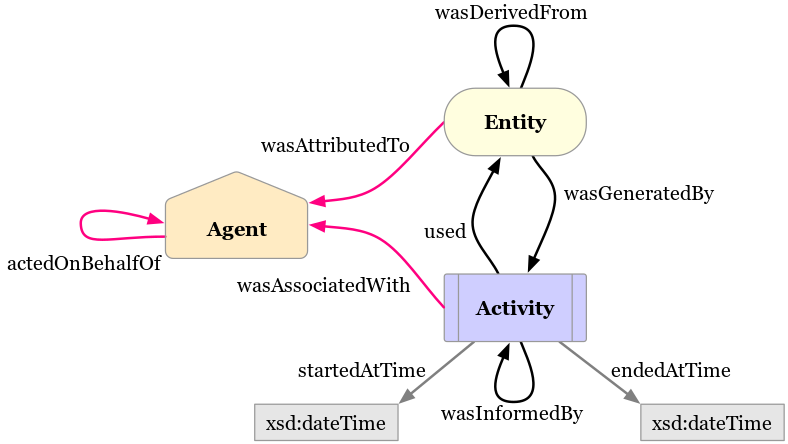
\includegraphics[width=0.8\linewidth]{img/prov-o-model.png}
    \caption{Overview of PROV-O model \cite{lebo_prov-o_2013}}
    \label{fig:prov-o-model}
\end{figure}

PROV-O is a generic and domain independent ontology for representing provenance information.
In order for it to be applied in domain of GDPR compliance, it needs to incorporate relevant terminology and enable distinction between different types of activities and entities.
Furthermore, PROV-O as a provenance ontology is intended to represent information about activities that have been executed in the past, and is therefore suitable to represent information only in the ex-post aspects.

While PROV-O does provide the concept of \texttt{Plan}\footnote{PROV-O defines a \textit{plan} as a set of actions or steps towards some goal. It clarifies on the lack of concepts relevant to plans as - ``\textit{There exist no prescriptive requirement on the nature of plans, their representation, the actions or steps they consist of, or their intended goals.''}} to represent ex-ante information, it does not provide further concepts or relationships to associate a plan with activities and entities\footnote{PROV-O provides the concept of \texttt{Association} which assigns responsibility to an agent for an activity and indicates that the agent had a role in the activity, which can include a \texttt{Plan} associated using the \texttt{hasPlan} property.}.
In order to adopt PROV-O and use \texttt{Plan} for representing ex-ante information for GDPR compliance, it needs to be extended with additional concepts and relationships.

\subsubsection{P-Plan - extending PROV-O Plans as Workflows}
P-Plan \cite{garijo_p-plan_2014} extends the concept of \texttt{Plan} in PROV-O towards representing scientific
workflows which enable creating a template of a `step' and linking it to executions of activities.
A \texttt{p-plan:Plan} is a subclass of \texttt{prov:Plan} and is composed of smaller activities or steps (\texttt{p-plan:Step}) that use and generate (as inputs or outputs) variables (\texttt{p-plan:Variable}).
An overview of relationship between PROV-O and P-Plan is described in \autoref{fig:p-plan-model}.
P-Plan enables representation of provenance information associated with both ex-ante and ex-post processes by representing them as scientific workflows. It also enables associating plans with their executions, thereby providing a link between ex-ante and ex-post provenance information.
\begin{figure}[htbp]
    \centering
    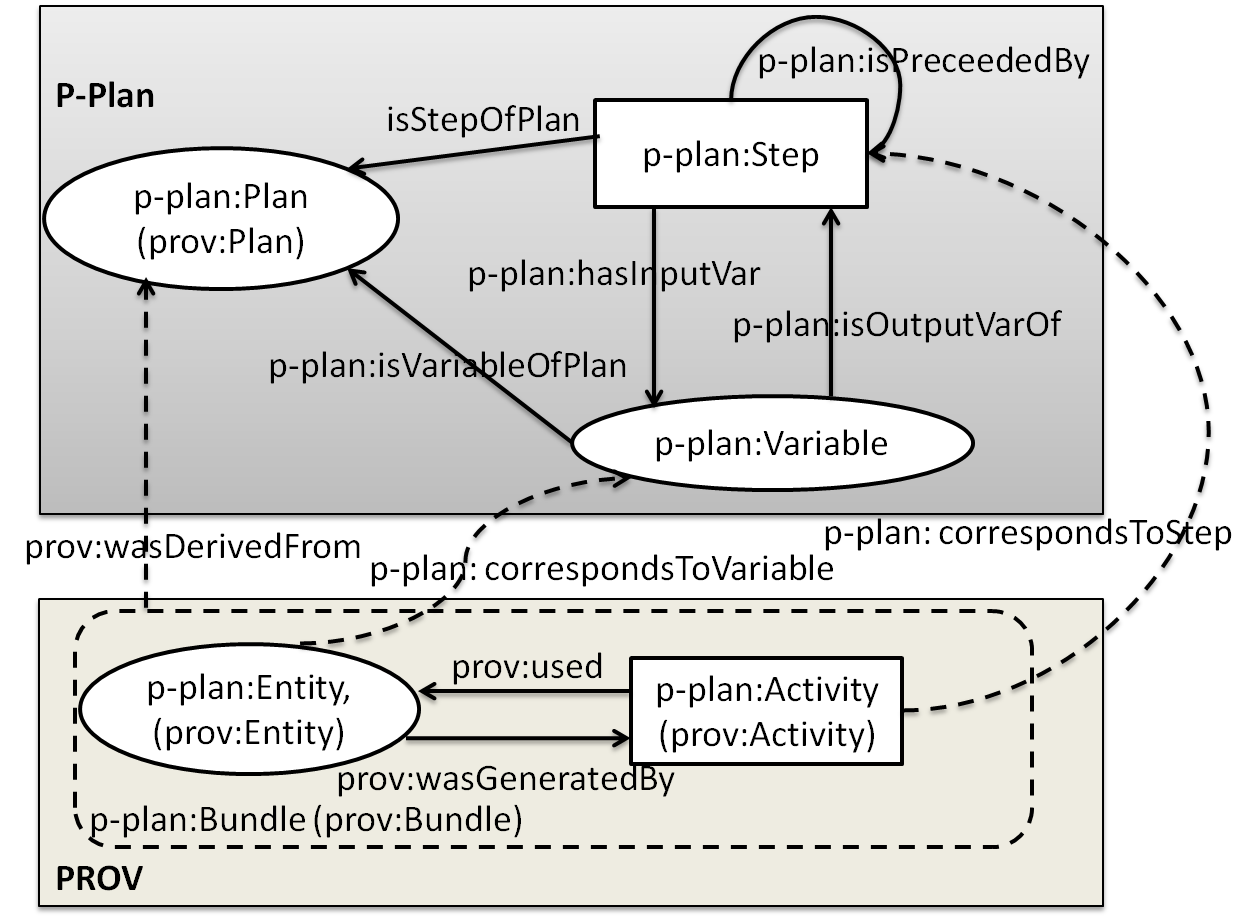
\includegraphics[width=0.75\linewidth]{img/p-plan-model.png}
    \caption{Overview of P-Plan model and its relationship with PROV-O \cite{garijo_p-plan_2014}}
    \label{fig:p-plan-model}
\end{figure}

A \texttt{p-plan:Plan} represents information of `how’ something should happen or a `template’ for executions. A \texttt{p-plan:Activity} is a subclass of \texttt{prov:Activity} and represents execution of process described in a \texttt{p-plan:Step}.
A \texttt{p-plan:Entity} is a subclass of \texttt{prov:Entity} that corresponds to a \texttt{p-plan:Variable} in \texttt{p-plan:Plan}. Therefore, a
\texttt{p-plan:Step} may describe the template including inputs and outputs which can
then be instantiated into multiple instances of \texttt{p-plan:Activity} that can have
distinct inputs to produce different outputs.
As \texttt{p-plan:Plan} extends \texttt{prov:Plan}, which itself extends \texttt{prov:Entity}, it can be
used to treat \texttt{p-plan:Plan} as an object whose provenance can be tracked using
PROV-O or P-Plan. This makes it possible to express `provenance of provenance' - thereby creating a record of how plans were formulated and executed over time.

\subsubsection{Extending ontologies for GDPR}
The PROV-O and P-Plan ontologies were extended to represent concepts and relationships of ex-ante and ex-post activities associated with personal data and consent based on requirements of GDPR compliance.
The decision to extend PROV-O and P-Plan with GDPR concepts was made as both ontologies contain generic concepts associated with activities and workflows which can be used for representing information about GDPR compliance, but doing so would be not be intuitive due to difference in terminology and structuring of information as expected for GDPR compliance.

Extending existing ontologies of PROV-O and P-Plan enables expressing a `template'
or `plan' using \texttt{p-plan:Plan} describing ex-ante activities (as \texttt{p-plan:Step}) that can take place. This template can then be used to denote execution of activities in ex-post phase using \texttt{p-plan:Activity}.
This provides a machine-readable and documented information model for both ex-ante and ex-post activities whose provenance itself can be expressed (using PROV-O and P-Plan) to record how they were created and how they  change over time.
This is beneficial in documenting state of a system at a given time through a set of activities that deal with consent and personal data, and
can be helpful in determining changes to be made based on changes in processing of personal data over time.

The extended ontology derived from PROV-O and P-Plan incorporates concepts and relationships associated with GDPR in order to normalise terminology for representing information associated with GDPR compliance.
Concepts and relationships are derived from competency questions and linked with relevant clauses within GDPR through using GDPRtEXT concepts using \texttt{rdfs:isDefinedBy} and \texttt{rdfs:seeAlso}.
This provides documentation regarding origin of concepts and their use in representation of information associated with specific clauses of GDPR.
It also provides a machine-readable link from the ontology to GDPR which can be used to compare, analyse, and align relevant ontologies.

The extension consists of sub-classing existing concepts in PROV-O and P-Plan to represent specific activities associated with GDPR compliance. 
The use of subclass mechanism preserves existing concepts and relationships of PROV-O and P-Plan to provide compatibility and reuse. This is particularly important for PROV-O as it is a W3C standard and therefore is more likely to have existing uses.
The compatibility with PROV-O also enables information defined using the ontology to be bundled as an artefact to record its provenance and planning as a form of meta-documentation regarding planning and maintenance of compliance activities This is particularly useful to maintain periodic snapshots of organisational processes associated with compliance and provides opportunities to automate querying and validation of information within a use-case - as demonstrated in \autoref{chapter:testing}.

\subsection{Ontology Description \& Application}
The ontology engineering is named GDPRov (GDPR Provenance Ontology) and is published online along with its documentation at \url{https://w3id.org/GDPRov/} under an open and permissive CC-by-4.0 license.
The ontology was created, documented, and published using the methodology presented in \autoref{sec:voc:methodology}.
The aim of GDPRov is to provide representations of ex-ante and ex-post activities regarding personal data and consent for GDPR compliance.
It uses GDPRtEXT concepts to define origin and relevance of its concepts to GDPR.

\subsubsection{Overview of GDPRov concepts}
GDPRov extends concepts from PROV-O and P-Plan using the sub-class and sub-property mechanisms to represent activities associated with GDPR compliance, with a visual overview provided in \autoref{fig:vocabs:gdprov-overview}.
\begin{figure}[htbp]
    \centering
    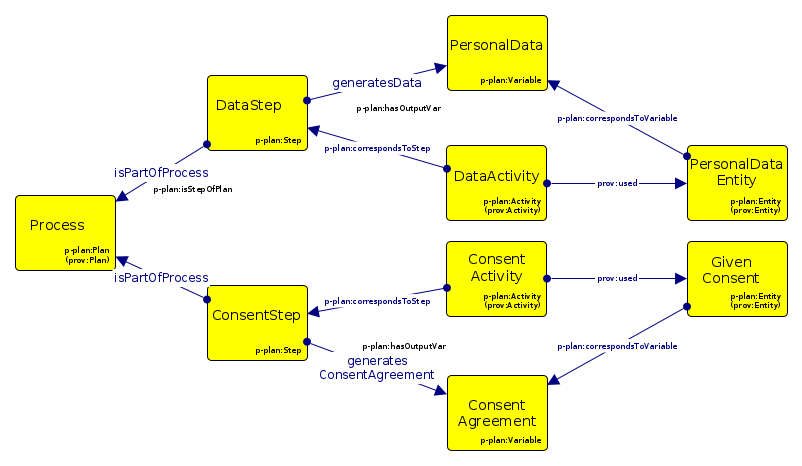
\includegraphics[width=\linewidth]{img/GDProv_relation_prov_pplan.png}
    \caption{GDPRov concepts derived by extending PROV-O and P-Plan}
    \label{fig:vocabs:gdprov-overview}
\end{figure}

GDPRov extends \texttt{p-plan:Plan} as \texttt{Process} to represent ex-ante plans of activities that will take place. The terminology is based on common use of term in expressions such as `business processes' and `compliance processes'.
Each \texttt{Process} can contain steps (represented by \texttt{p-plan:Step}) to represent activities that interact with data and agents.
To associate steps with a process, the property \texttt{p-plan:isStepOfPlan} is extended as \texttt{isPartOfProcess}.
Another additional property - \texttt{refersToProcess} is also used to enable referring to a process without being a part of it.
Similarly, to associate data (defined in P-Plan as \texttt{p-plan:Variable}) the properties \texttt{p-plan:hasInputVar} and \texttt{p-plan:isOutputVarOf} are extended for activities using inputs and producing outputs respectively.

Ex-post activities in P-Plan are represented by \texttt{p-plan:Activity}.
Data interactions with these activities is represented by \texttt{p-plan:Entity} and the properties \texttt{prov:used} and \texttt{prov:wasGeneratedBy} are used to indicate inputs and outputs respectively.
GDPRov defines steps to indicate automated execution and user interactions regarding collecting data from user (input) and providing data (output).
To indicate a legal basis associated with a process or a step, the property \texttt{hasLegalBasis} is provided.

\subsubsection{Depicting Data Life-cycle}
Activities associated with life-cycle of personal data constitute of collecting, processing or using it, storing, sharing, deleting, transferring, transforming, anonymise, and rectifying data. GDPR defines several more categories of actions in Article 4-2 in its definition of `processing'.
GDPRov provides broad and abstract processes to represent data access, data archival, data erasure, and data rectification given the need to execute these using one or more steps.
GDPRov provides representations of actions in ex-ante phase as \texttt{DataStep} which extends \texttt{p-plan:Step} and in ex-post phase as \texttt{DataActivity} which extends \texttt{p-plan:Activity}.
These are further extended to distinguish between data collection, data deletion, data sharing, data storage, data archival, data transfer, data transformation, data usage, and rectification of data.
A visual overview of steps describing a data life-cycle using GDPRov is provided in \autoref{fig:vocabs:gdprov-data-lifecycle}.
\begin{figure}[htbp]
    \centering
    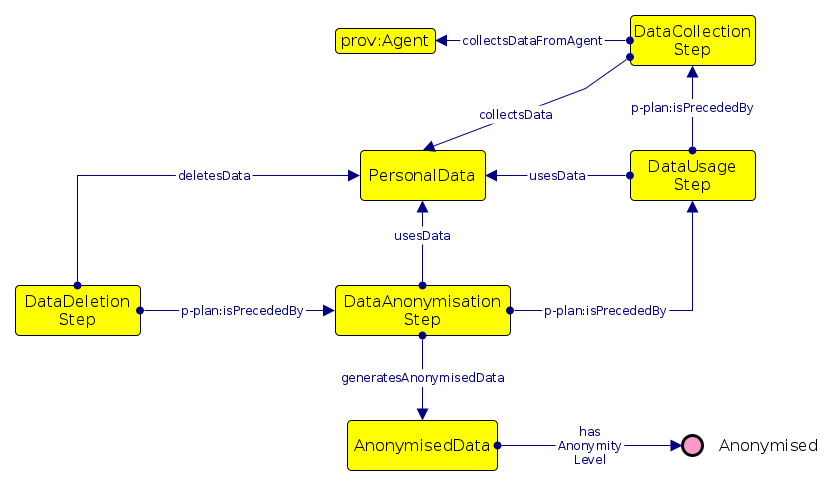
\includegraphics[width=\linewidth]{img/GDPRov_data_lifecycle.png}
    \caption{Example steps depicting data life-cycle using GDPRov}
    \label{fig:vocabs:gdprov-data-lifecycle}
\end{figure}

Anonymisation of data is defined as a sub-class of data transformation to indicate transformation of data that takes place when anonymising it.
As GDPR obligations are based on level of anonymity and capability of de-anonymising it from an organisation's point of view, GDPRov provides the concept of \texttt{anonymisation level} to indicate state of anonymity of data.
GDPRov defines four levels of anonymisation based on existing work in representing anonymous data \cite{hintze_meeting_2017}, which constitute of data that is: (i) completely anonymised, (ii) completely de-anonymised, (iii)pseudo-anonymised, and (iv) pseudo-organisational-anonymised where an organisation does not have additional data required to de-anonymise it and can thus utilise it internally as if it were completely anonymous data.
Sharing of data consists of interactions with actors or agents, which are represented by \texttt{prov:Agent} and associated with respective steps and activities using extended properties.

Personal data used within activities is represented by \texttt{PersonalData} which is sub-classed from \texttt{p-plan:Variable} for ex-ante representation and by \texttt{PersonalDataEntity} which is sub-classed from \texttt{prov:Entity} for ex-post representation.
Further categorisation of personal data into anonymised, sensitive, and representing user identifier is provided through sub-classes.

\subsubsection{Depicting Consent Life-cycle}
Activities associated with consent and its life-cycle are represented in ex-ante phase by sub-classing \texttt{p-plan:Step} as \texttt{ConsentStep} and in ex-post phase by sub-classing \texttt{p-plan:Activity} as \texttt{ConsentActivity}.
These are further sub-classed to represent acquisition, archival, modification, and withdrawal of consent.
Amongst these, withdrawal of consent is defined as sub-class of modification since it modifies state of consent.
A visual summary of steps in a consent life-cycle is provided in \autoref{fig:vocabs:gdprov-consent-lifecycle}.
\begin{figure}[htbp]
    \centering
    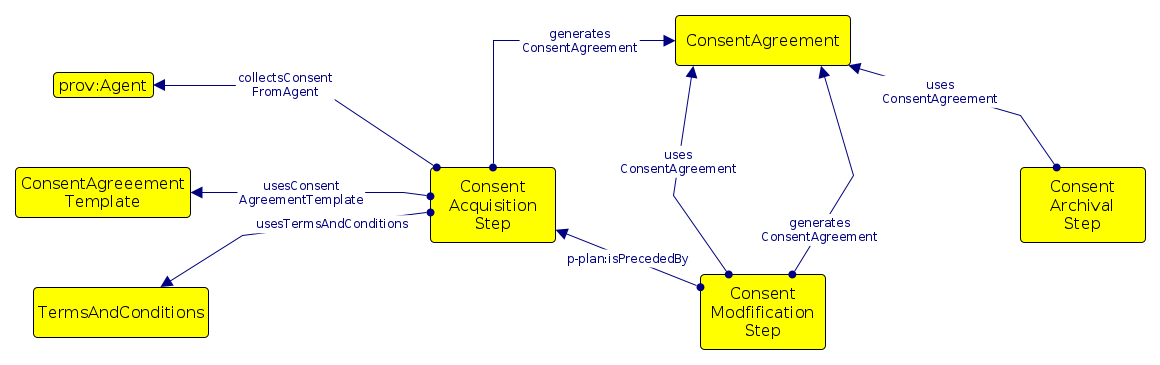
\includegraphics[width=\linewidth]{img/GDPRov_consent_lifecycle.png}
    \caption{Consent life-cycle defined using GDPRov}
    \label{fig:vocabs:gdprov-consent-lifecycle}
\end{figure}

Artefacts associated with consent and used in activities include choices or offer provided to request consent and subsequent consent given by an individual.
To represent these in ex-ante phase, GDPRov provides concepts of \texttt{ConsentAgreementTemplate} to represent template offered to collect consent, \texttt{ConsentAgreement} to indicate given consent, and \texttt{TermsAndConditions} to indicate applicable policies or terms and conditions.
Corresponding concepts in ex-post phase are \texttt{GivenConsentTemplate}, \texttt{GivenConsent}, and \texttt{TermsAndConditionsEntity}.

\subsubsection{Depicting Compliance-related processes}
In addition to representing activities associated with personal data and consent, GDPRov also provides representations for compliance-related processes.
These include actions such as appointing processor (by a controller), carrying out an impact assessment, marketing and its special case of direct marketing, and monitoring compliance.
Processes are also provided for handling data breaches which include notifying controller (by a processor), notifying data subject, and notifying data protection authority.
The handling of rights required by GDPR is represented through sub-classes of \texttt{Process} for data portability, erasure, access personal data, basic info about processing, no automated processing, object to direct marketing, object processing, rectification, restrict processing, transparency, SAR (subject access request).

% \subsubsection{Actors and Agents}
% Controller Representative
% Data Subject
% DPO
% Processor Representative
% Third Party
%     Controller
%         Joint Controller
%     Processor
%         SubProcessor

% \subsubsection{Documentation \& Dissemination}

\subsubsection{Example Use-Case: Querying anonymised sharing of data}
The applicability and usefulness of GDPRov is demonstrated through its use for querying and validation of information for GDPR compliance in \autoref{chapter:testing}.
A simplified example demonstrating a similar application through use of a SPARQL query was published along in a peer-reviewed publication \cite{pandit_modelling_2017}. It is presented in \autoref{code:gdprov:sparql} to demonstrate how GDPRov can assist in answering of compliance questions for GDPR.

The query uses GDPRov concepts to retrieve data being shared, specific steps that share it, anonymisation level of shared data, and steps used to anonymise it. The query is meant to retrieve information relevant in investigation of data being shared and its anonymity.
\begin{listing}[htbp]
\begin{minted}{sparql}
PREFIX gdprov: <https://w3id.org/GDPRov#>
SELECT ?data ?sharestep ?isAnonymised ?anonymisationStep
WHERE {
    ?data a gdprov:Data .
    ?sharestep a gdprov:DataSharingStep .
    ?sharestep gdprov:sharesData ?data. 
    BIND (
        EXISTS { ?data a gdprov:AnonymisedData . }
        as ?isAnonymised ) .
    OPTIONAL {
        ?anonymisationStep
        gdprov:generatesAnonymisedData ?data .
    }
}
\end{minted}
\caption{SPARQL query representing compliance question \texttt{G5} concerning legal basis for processing}
\label{code:gdprov:sparql}
\end{listing}

\subsubsection{Example Use-Case: Detecting changes in activities for updates to consent}
As an use-case, consider the case where a data controller updates a plan of processing activities - such as when a purpose changes or a new processing operation is added to an existing purpose, and where legal basis for such processing is consent.
In such cases, a data controller is required to evaluate whether updating an individual's consent is required based on changes between given consent and new purposes or processing activities. By storing plans of processing operations using GDPRov, it is possible to compare the old and new versions of a plan, detect changes, and identify whether corresponding updates to consent are needed. 

An exploration of above as change detection was published in Managing the Evolution and Preservation of the Data Web workshop co-located with ESWC 2018 \cite{pandit_gdpr-driven_2018}. It described comparison of plans represented using P-Plan to identify changes based on the above obligation. 

The change detection, visualised in \autoref{fig:vocabs:gdprov-change-detection}, is based on identifying differences between two plans in terms of steps and variables and whether they have been added, removed, or modified.
In the figure, the change reflects removal of a step - which by itself does not require any changes to given consent since no new purposes have been added to an existing given consent.
Using this approach, the detected change can be analysed - manually for complex and legal interpretations and automatically for simpler or simplified graphs - and used to identify whether corresponding changes are necessary based on compliance obligations.
\begin{figure}[htbp]
    \centering
    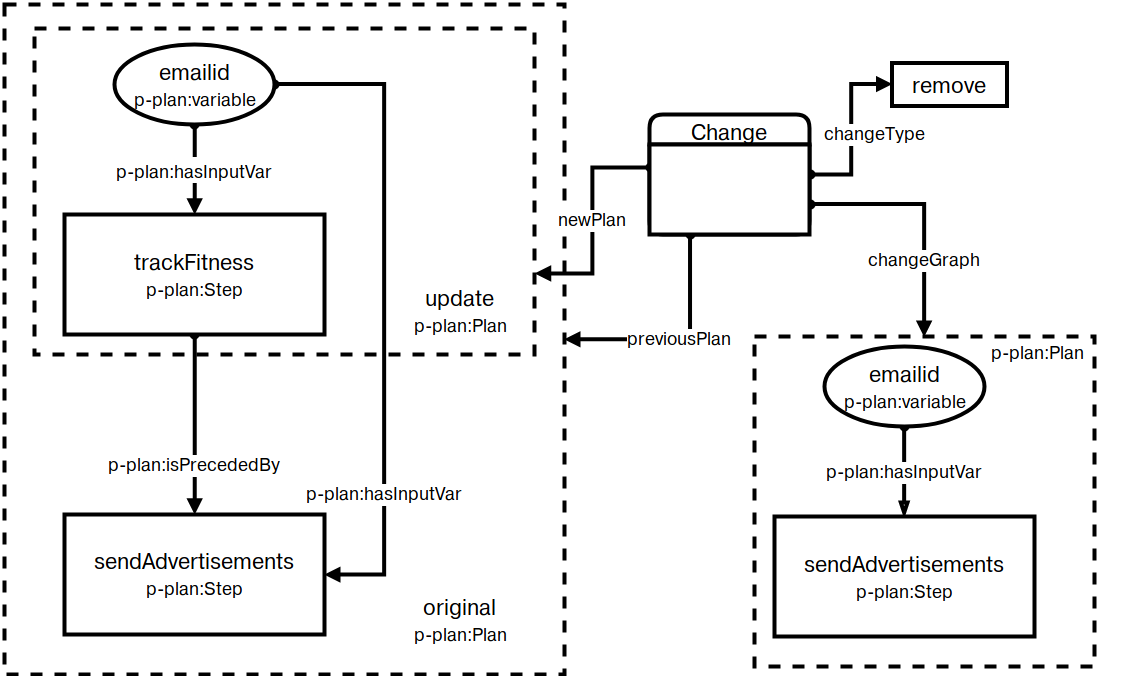
\includegraphics[width=\textwidth]{img/GDPRov-change-detection.png}
    \caption{Modelling changes in workflows using P-Plan \cite{pandit_gdpr-driven_2018}}
    \label{fig:vocabs:gdprov-change-detection}
\end{figure}

\subsection{Evaluation}\label{sec:voc:gdprov:evaluation}
The ontology assessment was based on the methodology outlined in \autoref{sec:voc:methodology} regarding criterion for ontology quality and documentation.
The ontology was used in two applications developed to demonstrate use of SPARQL to query information (see \autoref{sec:testing:sparql}) and SHACL to validate information for GDPR compliance (see \autoref{sec:testing:shacl}). The experience demonstrates suitability of GDPRov in representing the required information, and led to addition of \texttt{ConsentAgreementTemplateBundle} (in v0.7) as a concept for convenience in representing `bundled' consent requests and provisions based on consent workflows on a website where a single dialogue is used to collect consent involving multiple distinct purposes and third parties.

GDPRov was published \cite{pandit_modelling_2017} as a peer-reviewed publication in Workshop on Society, Privacy and the Semantic Web - Policy and Technology (PrivOn) co-located with the 16th International Semantic Web Conference (ISWC). The workshop provided reviews from domain experts in privacy, legal, and semantic web domains; with ISWC being a top-tier conference in semantic web domain.
As of February 2020, this publication has received 18 citations to (excluding self-citations) on Google Scholar\footnote{\url{https://scholar.google.com/scholar?cites=2287149512924017207}} of which 2 are deliverables of CitySPIN research project (see \autoref{sec:sota:gdpr-semweb}).
% Of these, the publications associated with PrOnto \cite{palmirani_pronto_2018,palmirani_pronto_2018-1} incorrectly conclude that ``GDPRov aims to describe the provenance of the consent and data lifecycle in the light of the Linked Open Data principles such as Fairness and Trust'' - since the basis of GDPRov is the scientific workflow model similar to the one used within PrOnto.
% The publication of a PROV-O model representing activities for GDPR compliance by Ujcich et al. \cite{belhajjame_provenance_2018} cites GDPRov as a relevant approach with the comparison to GDPRov specified as - ``Our model allows for more flexible specifications of how data can be used (i.e.,under consent for particular purposes while being legally valid for a period of time). Furthermore, our model focuses on temporal reasoning and online data usage control, whereas it is not clear how amenable GDPRov is to such reasoning or enforcement.'' While the example provided in the publication does provide temporal annotation of activities for GDPR compliance - these are achieved through the use of PROV-O rather than specialised classes using GDPR terminology. Since GDPRov extends PROV-O, it supports such use of inherent PROV-O concepts. In addition, GDPRov provides expression of ex-ante activities and workflows which cannot be expressed using the model proposed by Ujcich et. al.
A publication describing an approach for annotating DFDs (data flow diagrams) with information for analysing compliance \cite{debruyneOntologyRepresentingAnnotating2019} utilised GDPRov to represent personal data as an entity used in activities within its ontology for representing DFDs to abstract processing operations as data flows.

\subsubsection{Fulfilment of Competency Questions}
An assessment of the extent to which GDPRov satisfies competency questions by providing concepts and relationships is presented here as part of its evaluation.
The competency questions, summarised in \autoref{sec:gdprov:cq}, were used to guide development of ontology and therefore are used to evaluate the extent to which the developed ontology meets requirements of representing this information.
\autoref{table:gdprov:cq} lists concepts and properties for answering competency question (with \textit{N/S} used to indicate not in scope).
\begin{center}
    \footnotesize
\begin{tabularx}{\textwidth}{|l|X|p{5cm}|l|}
\caption{Concepts in GDPRov for answering competency questions} \label{table:gdprov:cq} \\
\toprule
\textbf{CQ} & \textbf{Class} & \textbf{Property} & \textbf{Phase} \\
\midrule
\endfirsthead

\caption*{Concepts in GDPRov for answering competency questions (cont'd)} \\
\toprule
\textbf{CQ} & \textbf{Class} & \textbf{Property} & \textbf{Phase} \\
\midrule
\endhead

\midrule
\multicolumn{4}{r@{}}{\footnotesize (Cont'd on following page)}\\
\endfoot

\endlastfoot


\multicolumn{4}{|l|}{\textbf{Actors and Agents involved in activities}}  \\ \hline
\textit{CMQ2} & \textit{Controller}, \textit{ControllerRepresentative}, \textit{DPO} &  &  \\ \hline
\textit{CMQ17} & \textit{Processor}, \textit{ProcessorRepresentative}, \textit{DPO} &  &  \\ \hline
\textit{CMQ35} & \textit{DataSubject} &  &  \\ \hline
\multicolumn{4}{|l|}{\textbf{Details of processing}}  \\ \hline
\textit{CMQ3} & \textit{Process} & \textit{refersToProcess} & \textit{Ex}-\textit{ante} \\ \hline
\textit{CMQ4} & \textit{DataSubject} &  &  \\ \hline
\textit{CMQ5} & \textit{PersonalData}, \textit{SensitiveData} & \textit{usesData} & \textit{Ex}-\textit{ante} \\ \hline
 & \textit{PersonalDataEntity}, \textit{SensitiveDataEntity} &  & \textit{Ex}-\textit{post} \\ \hline
\textit{CMQ6} & \textit{DataSharingStep} & \textit{sharesData}, \textit{sharesDataWith} & \textit{Ex}-\textit{ante} \\ \hline
 & \textit{DataSharingActivity} & \textit{hasSharedDataWith} & \textit{Ex}-\textit{post} \\ \hline
\textit{CMQ7} & \textit{ThirdParty} & \textit{sharesDataWithThirdParty} & \textit{Ex}-\textit{ante} \\ \hline
\textit{CMQ8} & \textit{ThirdParty} & \textit{sharesData}, \textit{sharesDataWith} & \textit{Ex}-\textit{ante} \\ \hline
\textit{CMQ9} & \textit{N}/\textit{S} & \textit{N}/\textit{S} &  \\ \hline
\textit{CMQ10} & \textit{N}/\textit{S} & \textit{N}/\textit{S} &  \\ \hline
\textit{CMQ11} & \textit{DataStorageStep} & \textit{usesData}, \textit{generatesData} & \textit{Ex}-\textit{ante} \\ \hline
 & \textit{DataStorageActivity} &  & \textit{Ex}-\textit{post} \\ \hline
\textit{CMQ12} & \textit{N}/\textit{S} & \textit{N}/\textit{S} &  \\ \hline
\textit{CMQ13} & \textit{N}/\textit{S} & \textit{N}/\textit{S} &  \\ \hline
\textit{CMQ26} &  & \textit{hasLegalBasis} &  \\ \hline
\multicolumn{4}{|l|}{\textbf{Lifecycle of data}} \\ \hline
\textit{CMQ28} & \textit{DataCollectionStep} & \textit{collectsData} & \textit{Ex}-\textit{ante} \\ \hline
 & \textit{DataCollectionActivity} &  & \textit{Ex}-\textit{post} \\ \hline
\textit{CMQ29} & \textit{DataCollectionStep} & \textit{collectsDataFromAgent} & \textit{Ex}-\textit{ante} \\ \hline
 & \textit{DataCollectionActivity} & \textit{collectedDataFromAgent} & \textit{Ex}-\textit{post} \\ \hline
\multicolumn{4}{|l|}{\textbf{Anonymisation}} \\ \hline
\textit{CMQ31} & \textit{DataAnonymisationStep}, \textit{AnonymisedData} &  & \textit{Ex}-\textit{ante} \\ \hline
 & \textit{DataAnonymisationActivity}, \textit{AnonymisedDataEntity} &  & \textit{Ex}-\textit{post} \\ \hline
\textit{CMQ32} & \textit{PersonalData}, \textit{SensitiveData} & \textit{hasAnonymityLevel} & \textit{Ex}-\textit{ante} \\ \hline
\multicolumn{4}{|l|}{\textbf{Activities associated with Consent}} \\ \hline
\textit{CMQ48} & \textit{ConsentStep}, \textit{ConsentAcquisitionStep}, \textit{ConsentModificationStep}, \textit{ConsentArchivalStep}, \textit{ConsentAgreement}, \textit{ConsentAgreementTemplate} & \textit{usesConsentAgreement}, \textit{generatesConsentAgreement} & \textit{Ex}-\textit{ante} \\ \hline
 & \textit{ConsentActivity}, \textit{AcquireConsentActivity}, \textit{ArchiveConsentActivity}, \textit{ModifyConsentActivity}, \textit{GivenConsent}, \textit{GivenConsentTemplate} & \textit{collectedConsentFromAgent} & \textit{Ex}-\textit{post} \\ \hline
\textit{CMQ49} & \textit{ConsentAgreementTemplate} &  & \textit{Ex}-\textit{ante} \\ \hline
 & \textit{GivenConsentTemplate} &  & \textit{Ex}-\textit{post} \\
\bottomrule
\end{tabularx}
\end{center}

% Some questions which were not considered in scope regarding expression of activities are marked with \textit{N/S}. 
Questions not in scope (marked as \textit{N/S} either require clarity from authoritative sources regarding interpretation of information to provide a concrete design pattern or have multiple possible representations of which it cannot be determined which is more useful from a legal compliance point of view. Examples include location of recipients - which can be expressed either through an property/annotation associated with a data sharing activity or attached with a particular third party; and specifying time limits or duration or conditional events associated with data storage and deletion periods. These have been identified as future work regarding further development of the ontology based on differing interpretations of representation, complexity of specifying values such as ``EU membership'' and  ``as long as required'', and pending expert opinion of legal authorities on these issues through courts or executive decisions.
These are considered minor issues regarding representation of information as they do not have a major impact on design and use of GDPRov.
Approaches and ontologies in SotA provide alternative design patterns which can be used as non-authoritative approaches for short-term mitigation of this issue.

The presented evaluation demonstrates GDPRov satisfies requirements of answering competency questions regarding representation of activities and identifies those that are needed to be resolved as future work based on availability of legal opinion and decisions. GDPRov thus fulfils research objective $RO3(b)$ by providing representations of activities associated with personal data and consent in ex-ante and ex-post phases.

\subsubsection{Comparison with SotA}
The representation of process flows and activities associated with GDPR compliance in existing approaches was presented and analysed as part of state of the art in \autoref{sota:analysis:process-flows}.
The attributes for this analysis involved features or concepts that could be represented using the specified approach and basis for representation in existing vocabularies and standards.
The analysis demonstrated existence of a variety of approaches that utilised  existing standards of PROV-O and BPMN to model GDPR-specific information regarding process flows and activities in both ex-ante and ex-post phase. It found that approaches modelling both ex-post and ex-ante phases exist and utilise PROV-O as their basis for representation of information.

A comparison of GDPRov with SotA is provided in \autoref{table:gdprov:sota} using the same attributes used for analysis.
The table lists features supported by each approach using a check mark (\cmark) with a blank indicating no information regarding the feature was found.
Column headings corresponding with expression of information supported by an approach, and use following abbreviations - (Repr): method used for representation of process flow; (EA): whether it permits Ex-ante modelling; (EP): whether it permits Ex-post modelling; (Pu): whether Purpose can be specified; (Pr): whether Processing can be specified; (DS): if Data Sharing can be modelled; (Rp): if Recipients are associated with data sharing; (St): whether Data Storage occurs; (Rg): if provision of Rights can be modelled; and (LB): if Legal Basis can be associated with a process flow.

The table demonstrates that GDPRov supports all of analysed features and is the only one currently providing all of them. However, this analysis only takes into consideration abstract existence or provision of features and does not take into consideration context of an approach or its granularity. For example, while an approach may provide representation of data storage concepts, there are additional features such as storage duration, condition, form or medium, security, and policy which are also relevant in evaluation of GDPR compliance.
These are highly dependant on individual use-cases and domains, and contain existing work which can be used to represent them such as Time ontology \cite{cox_time_2017} for temporal annotations and ODRL ontology \cite{iannella_odrl_2018} for conditions and events as policies.
Since the scope of GDPRov is limited to expression of information regarding activities in ex-ante and ex-post phases, representation of such granular attributes is relevant but not the primary focus within its scope and is therefore not considered in its evaluation or comparison with SotA.
% Table GDPRov vs SotA
\begin{center}
    \footnotesize
\begin{tabularx}{\textwidth}{|l|l|X|X|X|X|X|X|X|X|X|}
\caption{Comparison of GDPRov with SotA}\label{table:gdprov:sota} \\
\toprule
\textbf{Work} & \textbf{Repr} & \textbf{EA} & \textbf{EP} & \textbf{Pu} & \textbf{Pr} & \textbf{DS} & \textbf{Rp} & \textbf{St} & \textbf{Rg} & \textbf{LB} \\
\midrule
\endfirsthead

\caption*{Comparison of GDPRov with SotA (cont'd)} \\
\toprule
\textbf{Work} & \textbf{Repr} & \textbf{EA} & \textbf{EP} & \textbf{Pu} & \textbf{Pr} & \textbf{DS} & \textbf{Rp} & \textbf{St} & \textbf{Rg} & \textbf{LB} \\
\midrule
\endhead

\midrule
\multicolumn{11}{r@{}}{\footnotesize (Cont'd on following page)}\\
\endfoot
\endlastfoot

\rowcolor[gray]{0.8}
\textbf{GDPRov} & PROV-O,P-Plan & \cmark & \cmark & \cmark & \cmark & \cmark & \cmark & \cmark & \cmark & \cmark  \\ \hline
SPECIAL & PROV-O & \cmark & \cmark & \cmark & \cmark & \cmark & \cmark & \cmark &  &  \\ \hline
SPL+CitySPIN & PROV-O & \cmark & \cmark & \cmark & \cmark & \cmark & \cmark & \cmark &  &  \\ \hline
MIREL & PWO & \cmark &  & \cmark & \cmark &  &  & \cmark & \cmark &  \\ \hline
MRL+DAPRECO & PWO & \cmark &  & \cmark & \cmark &  &  & \cmark & \cmark &  \\ \hline
BPR4GDPR &  & \cmark & \cmark & \cmark & \cmark & \cmark & \cmark &  &  &  \\ \hline
Ujcich et al. & PROV-O &  & \cmark & \cmark & \cmark & \cmark & \cmark & \cmark & \cmark & \cmark \\ \hline
Lodge et al &  & \cmark &  & \cmark &  &  &  &  &  &  \\ \hline
Tom et al & BPMN & \cmark &  &  & \cmark & \cmark & \cmark & \cmark & \cmark &  \\ \hline
LUCE &  & \cmark & \cmark &  &  & \cmark & \cmark &  &  &  \\ \hline
Sion et al &  & \cmark &  & \cmark & \cmark & \cmark & \cmark & \cmark &  & \cmark \\ \hline
privacyTracker &  & \cmark & \cmark &  &  & \cmark & \cmark &  &  &  \\ \hline
Basin et al &  & \cmark &  & \cmark &  &  &  &  &  &  \\ \hline
RestAssured &  &  &  & \cmark & \cmark & \cmark & \cmark & \cmark &  &  \\ 
\bottomrule
\end{tabularx}
\end{center}

Regarding expression of information as being in either ex-ante or ex-post phase - GDPRov is the only approach to do so using existing ontologies of PROV-O and P-Plan based on a scientific workflow model which is useful in investigation of executions based on a plan and association of information between ex-ante and ex-post phases. The use of PWO \cite{gangemi_publishing_2017} in MIREL project also follows a similar rationale though it does not provide the same extent of concepts and representations as GDPRov.
In addition, utilisation of PROV-O as its base ontology enables information represented using GDPRov to be captured and recorded as provenance information using PROV-O or GDPRov itself. This provides capabilities for documenting evolution of a system as well as representing state of compliance at a given moment in time.
This feature is shared by all approaches that utilise a provenance based ontology at their core, and especially the ones that utilise PROV-O as it is a well-recognised and adopted standard.
The combination of PROV-O and P-Plan enables a flexible representation of activities by specifying their constituent steps and involved artefacts at an arbitrary level of granularity while providing annotations and classes to link these with GDPR. In this, GDPRov is unique and novel within SotA.

Based on this, GDPRov's novelty within SotA is based on it being one of few approaches using PROV-O to represent activities for GDPR compliance in both ex-ante and ex-post phases. GDPRov is also novel in its provision of concepts associated with GDPR and granularity afforded by use of PROV-O and P-Plan to link information in ex-ante and ex-post phases.
Furthermore, GDPRov is one of few approaches to be available under an open and permissive license (CC-by-4.0) thereby enabling its use, adoption, and further evolution.

\subsubsection{Application to external use-case from SPECIAL project}\label{sec:gdprov:use-case:SPECIAL}
% description of the use-case
The SPECIAL project uses a scenario\footnote{NOTE: the scenario explicitly mentions use of an immutable distributed ledger developed by the SPECIAL project to provide transparency and log accountability regarding metadata. This is omitted from the adapted use-case used to evaluate GDPRov.} to motivate their work and demonstrate use of developed technologies in their deliverables (D1.7 \cite{bonatti_d1.7_2018}) and peer-reviewed publications (\cite{kirrane_scalable_2018}).
In this section, the scenario is adapted as an external use-case to evaluate GDPRov's suitability to express required concepts.

The use-case is summarised as follows with GDPR concepts added in parenthesis for relevance: Sue (Data Subject) buys a wearable appliance for fitness tracking from BeFit (Data Controller), and is presented with an informed consent request that describes collection of biomedical parameters such as heart rate (Personal Data) and how they will be processed, which are stored in BeFit's cloud and transmitted for purposes of: giving Sue feedback on her activity, such as calories consumption; and creating an activity profile that will be shared with other companies for targeted ads related to fitness - an optional purpose to which Sue opts-in. After two years, Sue starts receiving annoying SMS messages from a local gym that advertise its activities. Sue discovers following facts: (i) the gym has an activity profile referring to Sue, that, due to appliance’s malfunctioning, reports that she is not doing any physical exercise; (ii) the gym received Sue's profile from BeFit, associated with a policy that allows the gym to send targeted ads to Sue based on the profile; (iii) BeFit built Sue's profile by mining data collected by appliance; and (iv) all these operations are permitted by consent agreement previously signed by Sue and BeFit. Using this information BeFit and the gym prove that they used Sue’s data in accordance with Sue's given consent. Sue now asks both BeFit and the gym to delete all of her data. 

The use-case is accompanied with information on its interpretation in terms of GDPR terminology \cite{bonatti_d1.7_2018} and its representation using  SPECIAL vocabularies \cite{kirrane_scalable_2018}. To represent the use-case using GDPRov, concepts used by SPECIAL are mapped or aligned to their closest relative concepts within GDPRov (see \autoref{table:gdprov:use-case:SPECIAL}) with its RDF/Turtle representation provided in \autoref{code:gdprov:use-case:special}. The SPARQL queries used to retrieve information depicted by statements (i) to (iv) in the scenario are provided in \autoref{code:gdprov:use-case:special-sparql}. The RDF representation and SPARQL query utilised a simplified representation of the scenario to present only the essential fact for answering of questions. 
\begin{center}
    \footnotesize
\begin{tabularx}{\textwidth}{|p{0.35\linewidth}|X|X|}
\caption{GDPRov concepts to represent external use-case from SPECIAL} \label{table:gdprov:use-case:SPECIAL} \\
\toprule
\textbf{Statement} & \textbf{GDPRov concept} & \textbf{SPECIAL concept} \\
\midrule
\endhead
Sue & \texttt{DataSubject} & \texttt{DataSubject} \\ \hline
BeFit & \texttt{DataController} & \texttt{Controller} \\ \hline
Biomedical parameters, heart rate, calories consumption, activity profile & \texttt{PersonalData} & \texttt{Data} \\ \hline
Collect data & \texttt{DataCollectionActivity} & \texttt{Collect} \\ \hline
Provide feedback on activity & \texttt{Purpose} & \texttt{Purpose} \\ \hline
Give consent (opt-in) & \texttt{AcquireConsentActivity} & \texttt{ConsentAssertion} \\ \hline
Targeted ads related to fitness & \texttt{Purpose} & \texttt{Purpose} \\ \hline
Share data & \texttt{DataSharingActivity} & \texttt{Recipient} \\ \hline
Gym & \texttt{ThirdParty} & \texttt{Recipient} \\ \hline
Consent agreement & \texttt{GivenConsent} & \texttt{LogEntryContent} \\ \hline
Delete data & \texttt{DataDeletionActivity} & N/A \\ \hline
Withdraw consent & \texttt{WithdrawConsentActivity} & \texttt{ConsentRevocation} \\
\bottomrule
\end{tabularx}
\end{center}
\begin{listing}[htbp]
\begin{minted}{turtle}
# Entities
:Sue a gdprov:DataSubject .
:BeFit a gdprov:DataController .
:Gym a gdprov:ThirdParty .
# Personal Data
:Biomedical_Parameters a gdprov:PersonalData .
:Activity_Profile a gdprov:PersonalData .

# Register with BeFit, given consent, and generate activity profile
:Registration a gdprov:Process .
:Sue_consent a gdprov:GivenConsent, gdprtext:LawfulBasisForProcessing .
:Collect_consent a gdprov:AcquireConsentActivity ;
    gdprov:isPartOfProcess :Registration .
    gdprov:collectedConsentFromAgent :Sue ;
    gdprov:generatedConsent :Sue_consent .
:Collect_data a gdprov:DataCollectionActivity ;
    gdprov:isPartOfProcess :Registration ;
    prov-o:wasInformedBy :Collect_consent ;
    gdprov:collectedDataFromAgent :Sue ;  # from Sue's device
    gdprov:generatedData :Activity_Profile .

# Share activity profile with Gym
:Targeted_ads_related_to_fitness a gdprov:Process ;
    gdprov:hasLegalBasis :Sue_consent .
:Share_data a gdprov:DataSharingActivity ;
    :sharedData :Activity_Profile ;
    :hasSharedDataWith :Gym .
# Gym receives Sue's activity profile from BeFit
:Collect_data_from_BeFit a :DataCollectionActivity ;
    gdprov:collectedDataFromAgent :BeFit ;
    gdprov:involvesAgent :Sue ;
    gdprov:refersToProcess :Targeted_ads_related_to_fitness ;
    gdprov:generatedData :Activity_Profile . # Gym copy of data

# Sue withdraws consent
:Withdraw_consent a gdprov:WithdrawConsentActivity ;
    prov:invalidated :Sue_consent .
# BeFit and Gym deleted the activity profile
:Delete_data a gdprov:DataDeletionActivity ;
    prov:invalidated :Activity_Profile ;
    prov:wasInformedBy :Withdraw_consent .
\end{minted}
\caption{GDPRov representation of external use-case from SPECIAL}
\label{code:gdprov:use-case:special}
\end{listing}
\begin{listing}[htbp]
\begin{minted}{sparql}
# Query (i)
# retrieves :Activity_Profile as personal data shared with Gym
# queried over Gym's records
SELECT ?personal_data 
WHERE {
    ?personal_data a gdprov:PersonalData .
    ?activity gdprov:generatedData .
    ?activity (gdprov:collectedDataFromAgent|gdprov:involvesAgent) :Sue .
}

# Query (ii)
# retrieves :BeFit as data source
# retrieves :Targeted_ads_related_to_fitness as purpose
# queried over Gym's records
SELECT ?party, ?purpose 
WHERE {
    ?activity gdprov:generatedData :Activity_Profile .
    ?activity gdprov:collectedDataFrom ?party .
    ?activity gdprov:refersToProcess ?purpose .
}

# Query (iii)
# retrieves :Sue as data source (as Sue's device)
# queried over BeFit's records
SELECT ?data_source 
WHERE {
    ?activity_profile gdprov:generatedData :Activity_Profile .
    ?activity_profile gdprov:collectedDataFromAgent ?data_source .   
}

# Query (iv)
# retrieves :Sue_consent as the legal basis for data collection and mining
# queried over BeFit's records
SELECT ?legal_basis 
WHERE {
    {
        ?activity gdprov:generatedData :Activity_Profile .
    } UNION {
        ?activity gdprov:sharedData :Activity_Profile .
        ?activity gdprov:hasSharedDataWith :Gym .
    }
    ?activity (
            gdprov:hasLegalBasis|
            (gdprov:isPartOfProcess/gdprov:hasLegalBasis))
        ?legal_basis .
}


\end{minted}
\caption{SPARQL queries using GDPRov for external use-case from SPECIAL}
\label{code:gdprov:use-case:special-sparql}
\end{listing}

Through the representation of concepts within the scenario and use of SPARQL, GDPRov is shown to support representation and answering of questions within the scenario. While the scenario relies on use of SPECIAL's policy-based vocabulary and immutable distributed ledger to store and retrieve information regarding given consent and processing activities carried out by BeFit and the Gym, these have not been replicated as storage mechanisms are not relevant within the use-case as adapted for this work.

One important conclusion from the above exercise is regarding representation of given consent where SPECIAL vocabularies represent given consent as a policy using OWL2 \cite{kirrane_scalable_2018}.
In comparison, GDPRov does not represent information provided within consent requests and given consent, but instead records its activities and associates generated consent as an artefact representing a legal basis with purposes (specified using \texttt{gdprov:Process}) that rely on it. 
This is the consequence of GDPRov focusing on representation of activities which does not concern representation of consent.
A consent-centric representation of this same scenario is presented in \autoref{sec:gconsent:use-case:SPECIAL} which uses GConsent to represent the scenario as interactions between consent states.

% \subsubsection{Application to external use-case from Ujcich et al.}
% Ujcich et al. present a similar (to the above) scenario in their demonstration of a provenance vocabulary based on the GDPR \cite{belhajjame_provenance_2018}. 
% The scenario concerns Alice, a customer, who registers with a retailer and provides name, address, and credit card number; gives consent to store these and use for purchases made, and also consents to use of name and address to receive marketing. 
% At some period of time, the retailer employs a third-party for marketing and provides it with Alice’s name and address based on the given consent.
% After some more period of time, Alice no longer wishes to receive marketing and withdraws her consent.
% The investigation of compliance presented in the publication utilises two questions related to the scenario, which are: (i) Was Alice’s personal data used for marketing purposes after Alice withdrew her consent?; and (ii) Was Alice’s personal data used for marketing purposes after Alice withdrew her consent?

% Ujcich et al. represent the scenario as a series of activities using PROV-O

% % breakdown into requirements
% % select concepts from GDPRov to represent requirements - ex-ante and ex-post
% % representation Turtle code
% % analysis - what is possible and what isn't
% % comment on deficiencies or advantages of GDPRov

% \subsubsection{Application to External Use-case: Ujcich et al.}
% % description of the use-case
% % breakdown into requirements
% % select concepts from GDPRov to represent requirements - ex-ante and ex-post
% % representation Turtle code
% % analysis - what is possible and what isn't
% % comment on deficiencies or advantages of GDPRov

\subsection*{Summary}
GDPRov is part of the second major contribution of this thesis. It provides an ontological representation of ex-ante and ex-post activities associated with personal data and consent for GDPR compliance.
It thus fulfils research objective $RO3(b)$ as outlined in \autoref{sec:intro:RQ}. 
The use of GDPRov makes it possible to indicate plans associated with how personal data and consent is collected, used, stored, shared, and erased.
It also enables representation of logs for activities that act over personal data and consent.

when GDPRov was first being developed (in 2016-2017), no other vocabulary was found that represented information about activities associated with GDPR compliance.
The work presented as state of the art in \autoref{chapter:sota} and demonstrating existence of approaches for representing information about GDPR processes were published after development and publication of GDPRov \cite{pandit_modelling_2017}. Of these approaches, some also utilise PROV-O to represent provenance of activities as found as presented in \autoref{sota:analysis:process-flows}. The differentiating factor of GDPRov is in use of PROV-O and P-Plan as distinct ontologies representing ex-ante and ex-post phases of activities based on a scientific workflow model - which is novel within state of the art. Another differentiating factor is use of GDPRtEXT to define origin and relevance of concepts to their basis in GDPR.

Approaches within state of the art, such as SPECIAL (\autoref{sec:sota:SPECIAL}), demonstrate applicability of provenance vocabularies in maintaining, querying, and assessing provenance logs represented using PROV-O for GDPR compliance.
While SPECIAL also provides ex-ante compliance assessment by using the same data model and logs it as a consent request instead of processing or execution \cite{dullaert_d3.4_2019}, GDPRov expands further on use of provenance to include representation of plans or templates to indicate association between activities in ex-ante and ex-post phases of compliance.

% GConsent
\section{GConsent - Ontology of Consent Information for GDPR Compliance}\label{sec:voc:GConsent}
GConsent is a semantic web ontology for representing contextual information about consent based on requirements of GDPR compliance. 
GConsent aims to model context, state, and provenance of consent as an entity.
Its scope is limited to consent as defined in GDPR and is intended towards assisting in modelling and management of information associated with compliance.
It uses GDPRtEXT to denote origin and relevance of its concepts within GDPR.

GConsent is the outcome of applying the methodology presented in \autoref{sec:voc:methodology} to identify and represent information about consent and its life-cycle as required to determine compliance with GDPR.
For this, information presented in \autoref{chapter:background} was used to identify validity of consent with requirements and compliance questions presented in \autoref{chapter:information} used as competency questions.
The latest iteration of GConsent (v0.5) is published online\footnote{\url{https://w3id.org/GConsent}} with its documentation under an open and permissive license of CC-by-4.0 and its code repository\footnote{\url{https://github.com/coolharsh55/GConsent/}}.

The design of GConsent was influenced by a real-world use-case for managing consent information based on GDPR compliance requirements, as mentioned earlier in \autoref{sec:info:compliance-questions-methodology}.
The design of ontology underwent several iterations based on whether it should model an association or dependency between purposes and processing operations associated with consent. The outcome, representing a decision and which is presented here, models separation between purpose and processing operations similar to other representations of consent within SotA.

\subsection{Distinction with existing work in state of the art}
Information about consent needs to be maintained and shared by multiple parties which includes data subjects who give consent, controllers who use it as legal basis, and authorities who evaluate its validity. GDPR requires information about consent across its life-cycle to be maintained, with an representation that is interoperable assisting all stakeholders in the compliance process - as outlined earlier in \autoref{sec:info:model}.

From existing work analysed in \autoref{chapter:sota}, the focus of approaches for consent is mostly on concept of `given' consent i.e. consent provided by a data subject and used as legal basis by a controller. There is a lack of work regarding representing other `states' of consent within its life-cycle as an entity or representation of agreement which are relevant to its use as legal basis in determination of processing of personal data and its compliance under GDPR.
Examples of such states are `not given', `refused', `withdrawn' which cannot be modelled in the same manner as `given consent' as they do not reflect the same information as given consent, but are still relevant when associated with a particular instance of processing. The state of a consent reflects its status for use as legal basis and is also relevant in management of consent information from an organisation's perspective.

Apart from the notion of states, existing approaches also lack modelling representations for events such as delegation, and associations with third parties regarding consent which have an effect on its validity regarding compliance.
GConsent aims to fill this gap, and therefore to provide novelty and contribution by representing a more cohesive and complete representation of information associated with consent for GDPR.

\subsection{Relationship with GDPRov}
GConsent builds upon and is complimentary to the representation of consent in GDPRov.
The definition of consent as an entity involved in activities is sufficient to express its life-cycle and provenance by using GDPRov. This includes ex-ante representation of information provided to collect consent and its subsequent agreement by an individual to produce given consent - which is then used within activities as a legal basis and may be modified, withdrawn, or revoked - signalling its effective end of life-cycle.
While GDPRov is sufficient to represent these states of consent as an entity along with information about activities acting on it, the primary focus of GDPRov is for expressing information regarding its association with activities.
Managing consent as a legal basis involves consideration of information such as purpose of processing, recipients, and contextual information such as medium of provision and collection, and situations such as delegation - which are not modelled in GDPRov.

GConsent aims to provide a consent-centric representation of these information categories by providing concepts relevant to resolution of valid consent as defined by requirements of GDPR compliance. In this, use of provenance concepts show an overlap with GDPRov.
This is resolved through differing scopes of the two ontologies, where concepts defined within GDPRov can also be defined using corresponding concepts in GConsent and vice-versa. An example of such cohesive usage is demonstrated through application of both GDPRov and GConsent for querying and validation of information in \autoref{chapter:testing}.
By having separation between GDPRov and GConsent, the ontologies are modular in their scope and concepts, and provide an adopter with choice regarding inclusion of semantics represented by each ontology.

\subsection{Requirements Gathering and Establishment of Competency Questions}
The scope of consent as represented within GConsent is limited to definition of consent as provided by Article 4-11\footnote{In this definition, consent is expressed as the indication of a data subject's wishes regarding processing of their personal data. However, this is a legal definition rather than a semantic one as it essentially defines the set of conditions required to be satisfied by some consent before it is considered valid under GDPR. Additionally, `consent' as a social concept has a pre-defined meaning based on its use in the social context. Therefore, referring to consent in the context of GDPR does not only mean given consent but includes all information and states associated with consent which can then be evaluated to assess whether it fits the definition of consent as a legal basis. Technical approaches can use `consent' to indicate the given consent or the set of all consent states within its life-cycle.} of GDPR. 
Other special cases of consent not included within GConsent consist of consent defined by Article 9 regarding use of special categories of personal data, Recital 33 regarding use of personal data for scientific research, and Article 8 along with Recital 38 regarding use of children’s personal data.
These were not included within the scope due to their additional requirements and complexity regarding interpretation and representation using semantic web. Additionally, current lack of real-world use-cases reflecting how these types of consent would function and legal guidance on their compliance requirements is noticeably absent in context of GDPR.

GConsent is primarily based on notion of consent as a legal basis under Article 6 of the GDPR. The conditions defined in Article 7, Recital 42, and Recital 43 provide requirements for consent to be considered or determined valid as per requirements of GDPR.
The Data Controller bears burden of demonstrating proof and satisfaction of requirements for consent to be considered valid as per Recital 42. This requires demonstrable proof that data subject provided consent and that it was valid as per obligations specified in GDPR.

For consent to be informed it is necessary to provide information to data subjects which includes specific purposes of processing the personal data.
GDPR also provides data subjects with right to modify or withdraw consent as defined in Article 7-3.
When consent is withdrawn, processing carried out done prior to withdrawal is considered valid under given consent in effect as legal basis during that period of time.

Through this, a rudimentary summary of information or attributes associated with `consent' as defined by GDPR is expressed as:
\begin{itemize}
    \item Data Subject the consent is about
    \item Personal Data associated with consent
    \item Processing operations or categories the consent is about, with data storage and data sharing having additional information requirements
    \item Purposes the consent is about
    \item Entity/Agent/Actor the consent is provided to
    \item Recipients of data or categories of recipients if any
\end{itemize}
These attributes are sufficient to provide a simplified representation of consent, and are used in existing approaches within state of the art - such as model of consent in SPECIAL vocabularies \cite{bonatti_special_2018}. However, these attributes are not sufficient by themselves to determine validity of consent as they lack information about context the consent was given in as well as changes to its state.

Therefore, further attributes associated with consent are identified and expressed as:
\begin{itemize}
    \item Entity/Agent/Actor that provided consent - relevant in case of delegation
    \item Entity/Agent/Actor that revoked, withdrew, or invalidated consent - relevant in case of delegation, and authoritative actions such as by regulators or courts
    \item Status of consent at a given period in time
    \item Contextual information regarding request and giving of consent such as - location, medium, timestamp, expiry
    \item Contextual information regarding revocation, withdrawal, and invalidation of consent such as - location, medium, timestamp, expiry
\end{itemize}
In addition to these, provenance information regarding how consent was requested and obtained is also important.
Specifically, information about specific processes and artefacts used in provision of request for consent should be recorded as they must satisfy GDPR qualitative requirements - such as request being clearly stated and being unambiguous.

To derive required concepts, competency questions were identified from compliance questions presented in \autoref{sec:info:compliance-questions} pertaining to given consent (\texttt{CMQ35-CMQ69}) and change in consent state (\texttt{CMQ70-CMQ87}).
These refer to information regarding consent (e.g. \texttt{CMQ35-CMQ40}), how consent was created/given/changed/invalidated (e.g. \texttt{CMQ41-CMQ52}), context of how consent was created/given/invalidated (e.g. \texttt{CMQ53-CMQ56}), and third parties associated with consent (e.g. \texttt{CMQ57-CMQ58}).

\subsection{Ontology Description \& Application}
\subsubsection{Core Concepts}
Core concepts and relationships in GConsent describe common and primary attributes associated with consent.
In this case, `consent' by itself does not refer only to state of `given consent' but also stands as a representation of `consent' as an entity whose state is unknown or is refused, withdrawn, or invalidated by Data Subject, Controller, or an authority such as courts. This definition of consent is based on managing consent as a data entity rather than as a semantic concept pertaining to an agreement by an individual. 
Core concepts are associated with consent in all its states and refer to information necessary to express what the consent is about. This comprises of the 5 attributes visualised in \autoref{fig:vocabs:gconsent-core} - Data Subject, Personal Data, Purpose, Processing, and Status.
\begin{figure}[htbp]
    \centering
    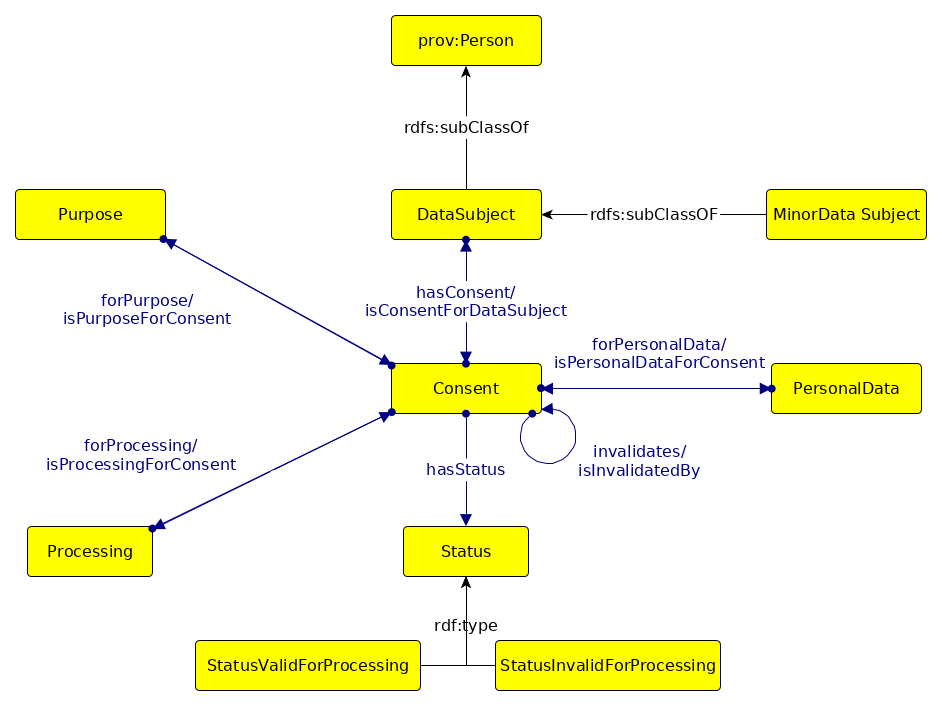
\includegraphics[width=0.8\linewidth]{img/gconsent_core.png}
    \caption{Core concepts in GConsent \cite{pandit_gconsent_2019}}
    \label{fig:vocabs:gconsent-core}
\end{figure}

\texttt{DataSubject} is natural individual consent is associated with as an agreement of their choices. This individual may or may not be the same entity that gave consent - as in case of parent or guardian giving consent for a child or as an act of delegation. \texttt{DataSubject} class is defined as a subclass of \texttt{prov:Person}, and with subclass \texttt{MinorDataSubject} to denote a data subject that is legally a minor or a child.
Each instance of \texttt{Consent} must be associated with one and only one \texttt{DataSubject}, and any further changes or modifications to a state of consent will continue to be associated with the same \texttt{DataSubject}.
\texttt{PersonalData} is a set of personal data associated with consent. Where multiple personal data are associated with a single instance of consent, it is interpreted to mean union of these sets of personal data. Similarly, multiple \texttt{Purpose} and \texttt{Processing} associated with a consent are also to be interpreted as union rather than intersection.
The `status' or `state' of consent indicates suitability of using that specific instance of consent as a legal basis for processing of personal data as defined by associated attributes.

\texttt{Purpose} and \texttt{Processing} are concepts that have semantic meaning based on their use within GDPR.
`Processing' is defined by Article 4-2, while `Purpose' has no specific definition provided but can be summarised as intent or aim of why the set of personal data is needed or to be used for. In practice, purpose is generally defined at a higher abstract level, and often encompasses several types or categories of data. An example of this is a privacy policy specifying `account information' and `location of service use' - which are data categories, that are `collected' and `used' - which are processing operations on personal data, `to ensure security of the account' - which is the purpose personal data will be processed for. The relation between a purpose and its associated processing operations is quite opaque when considered for purposes involving one or more processing operations. Based only on the description, it is difficult to determine which processing operations a purpose entails and vice versa, and their usage may not always be implied or commonly understood. Therefore, GConsent provides purpose and processing as self-declarative high-level concepts which can be extended with additional information for granularity and transparency.

\subsubsection{Context of Consent}
The context of consent refers to attributes such as location or time when instance of consent was created, invalidated, generated, changed, modified, given, or recorded.
GConsent provides concepts for expressing location, medium, and timestamp to indicate instant of creation or invalidation along with capturing `expiry' of consent as either an instant of time or a duration using Time vocabulary \cite{cox_time_2017}. The context also represents how consent was `provided' by a Person or Data Subject or Delegation. 
The provided contexts in GConsent are visualised in \autoref{fig:vocabs:gconsent-context}.

Context is associated with an instance of consent using generic property \texttt{hasContext}, with specialised properties extending it to indicate provision, expiry, location, time, and medium. 
Additional contexts can be represented and associated by extending \texttt{hasContext} in a similar manner.
\begin{figure}[htbp]
    \centering
    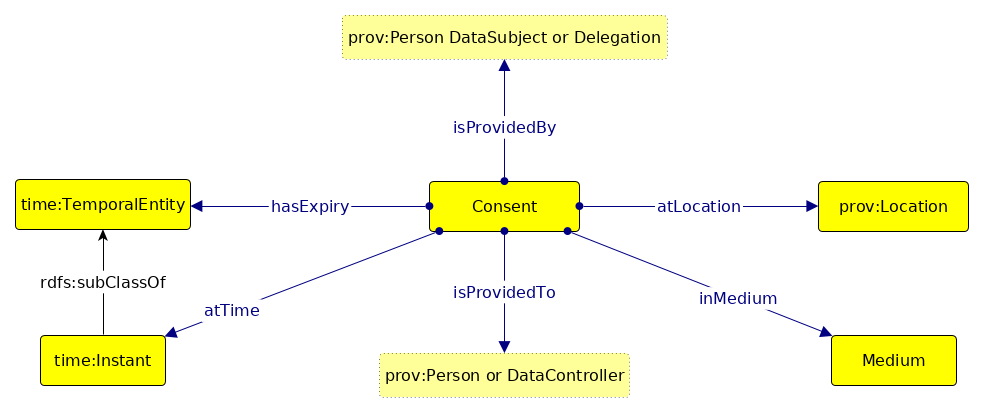
\includegraphics[width=0.8\linewidth]{img/gconsent_context.png}
    \caption{Concepts for representing context of consent in GConsent \cite{pandit_gconsent_2019}}
    \label{fig:vocabs:gconsent-context}
\end{figure}

\subsubsection{Consent States}
The state of consent determines suitability of its usage as a legal basis in  processing of personal data.
From a compliance perspective, there are only two categories of states - one which permits legal processing of personal data, and other being insufficient or prohibitive for processing.
GConsent represents these concepts by sub-classing \texttt{Status} as \texttt{StatusValidForProcessing} and \texttt{StatusInvalidForProcessing} to indicate use of a consent instance as valid or invalid legal basis as depicted in \autoref{fig:vocabs:gconsent-status}.
Instances provided to represent states of valid consent to indicate legal processing include - explicitly given, implicitly given, and given by delegation.
Instances provided that represent invalid states of consent to indicate processing should not be carried out include - unknown, not given, withdrawn, expired, invalidated, refused, and requested.

The use of state refers to tracking consent of a data subject from a legal perspective, and is aimed to aid in management of consent as an entity. For example, `unknown' reflects a situation where status of consent is not known - which can occur when importing consent information from another source.
This is distinct from `not given' which indicates an offer has been made for obtaining consent but a data subject has not yet provided any actionable response that could indicate acceptance or refusal - which are themselves represented by  states `given' and `refused' respectively.
For meeting obligations and requirements of GDPR compliance, it is not necessary to represent consent instances with states such as unknown or refused.
GConsent provides them for practical management of consent information where a controller may wish to track consent status of its processing operations throughout its life-cycle.
\begin{figure}[htbp]
    \centering
    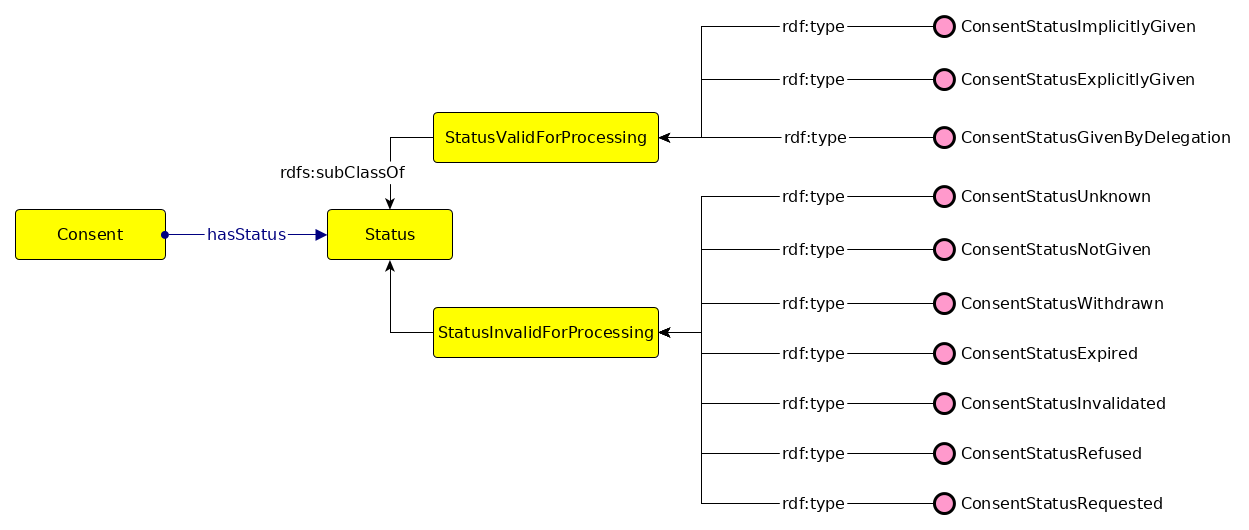
\includegraphics[width=\linewidth]{img/gconsent_status.png}
    \caption{Concepts representing state/status of consent in GConsent \cite{pandit_gconsent_2019}}
    \label{fig:vocabs:gconsent-status}
\end{figure}

GDPR requires keeping track of state change for consent - for example when status changes from given to withdrawn or when consent is invalidated because by a controller or legal authority. Whenever a consent status changes, this results in a new consent instance being created, which also assists in capturing context of the consent (such as time instant). This leads to a chain of consent instances, where `latest' consent is at `end' of this chain and indicates most recent operation regarding consent states. It is vital to record such provenance to demonstrate past processing was in compliance with state of consent at that point in time and to show changes to consent as part of its life-cycle.

\subsubsection{Example Use-Case}
The documentation of GConsent provides example applications in four use-cases to demonstrate how information can be represented, which are - (i) change in consent state, (ii) capturing given consent, (iii) capturing consent given via delegation, and (iv) capturing consent when data is shared with a third party.
The fourth use-case is presented here to demonstrate application of GConsent and use of its concepts to represent information towards GDPR compliance.

The example, visually represented in \autoref{fig:vocabs:gconsent-example}, shows association of a third party in role of a data processor\footnote{Under GDPR, a processor is not considered a third party, but has its own defined role as an entity associated with the Controller. However, from a lay person's perspective, the individual is the first party, the Controller is the second party, and any other entity is a third party. GConsent reflects this use in its structuring of entities where a Processor is considered a special type (sub-class) of Third Party.}
with whom data is shared for purposes of advertising. The association is captured by instance \texttt{ex:AdvertisingArrangement} of type \texttt{prov:Association}, and has \texttt{ex:AdPartner} defined as a \texttt{gdprov:Processor} defined with role as \texttt{gdprtext:Processor}. It is also possible to list out specific arrangement for this association using \texttt{prov:hadPlan} property and a \texttt{gdprov:Process} instance to list specific steps and entities involved in data sharing arrangement.

The example serves to demonstrate practical use of GConsent in representing information about consent, where PROV-O is used to specify relationships with a Processor. GConsent can be combined or supplemented with other ontologies to define such associations and practical reflections of data sharing agreements between parties. The defined instance of consent in example enables a Controller to track state of consent as the data subject is provided with choice of whether to agree to this arrangement or to refuse it, where upon agreement the option to exercise right to modify and withdraw consent is also provided.
\begin{figure}[htbp]
    \centering
    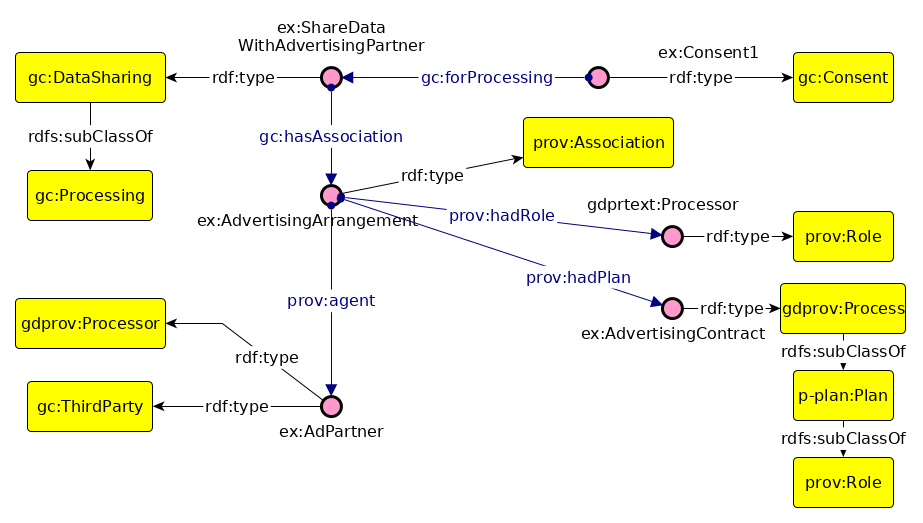
\includegraphics[width=0.8\linewidth]{img/gconsent_third_party_datasharing.png}
    \caption{GConsent representation of use-case involving third party data sharing \cite{pandit_gconsent_2019}}
    \label{fig:vocabs:gconsent-example}
\end{figure}

\subsection{Evaluation}\label{sec:voc:gconsent:evaluation}
GConsent as an ontology was evaluated regarding its capability to express information about consent using the methodology outlined in \autoref{sec:voc:methodology}.
This was an iterative process where the ontology was tested and modified to accommodate the requirements of the competency questions. Changes were made to the ontology where information was found to be missing or incorrectly modelled.
In particular, the iterations consisted of the degree and design of representing a dependency between purposes and processing operations associated with consent. These were ultimately rejected with the final iteration modelling purpose and processing independent of each other to provide greater granularity and reuse of these concepts.
An application of GConsent towards representation of consent information for a real-world website in the application of SHACL to validate information for GDPR compliance is presented in \autoref{sec:testing:shacl}.

GConsent was published in Extended Semantic Web Conference (ESWC) as a peer-reviewed publication \cite{pandit_gconsent_2019} in the Ontologies and Reasoning Track. As ESWC is a top-tier semantic web conference with a rigorous review process, acceptance of GConsent demonstrates its contribution as a semantic web resource.
Along with this, the documentation of GConsent, available online, also provides extensive information about the ontology and its potential applications. It also provides a brief comparison of the ontology with relevant approaches within state of the art.
GConsent, along with Consent Receipt standard \cite{lizar_consent_2017}, had a direct impact on design and development of consent information within DPV. In particular, GConsent provided concepts for expression of consent based on the GDPR and competency questions for integrating those with rest of DPV.
As of February 2020, GConsent does not currently have any citations (excluding self-citations) given recency of its publication.

\subsubsection{Fulfilment of Competency Questions}
Assessment of the extent to which GConsent provides concepts and relationships to answer competency questions is presented in \autoref{table:gconsent:cq}. 
In these, the PROV-O and Time ontologies are used in conjunction with GConsent to represent provenance and temporal information about consent and changes to it.
PROV-O is also used to capture association and roles of entities in activities associated with consent.
Based on these, GConsent satisfies requirements of providing information for answering compliance questions regarding consent and thus fulfils research objective $RO3(c)$.
\begin{center}
    \footnotesize
\begin{tabularx}{\textwidth}{|p{1cm}|X|p{4cm}|p{3.5cm}|}
\caption{Concepts in GConsent for answering competency questions} \label{table:gconsent:cq} \\
\toprule
\textbf{CQ} & \textbf{Question} & \textbf{Concepts} & \textbf{Properties} \\
\midrule
\endfirsthead
\caption*{Concepts in GConsent for answering competency questions (cont'd)} \\
\toprule
\textbf{CQ} & \textbf{Question} & \textbf{Concepts} & \textbf{Properties} \\
\midrule
\endhead

\midrule
\multicolumn{4}{r@{}}{\footnotesize (Cont'd on following page)}\\
\endfoot
\endlastfoot

\multicolumn{4}{|l|}{\textbf{Questions about consent}} \\ \hline
\textit{CMQ35} & Who is the consent about? & \textit{DataSubject} & \textit{isConsentForDataSubject} \\ \hline
\textit{CMQ36} & What type of Personal Data are associated with the Consent? & \textit{PersonalData} & \textit{forPersonalData} \\ \hline
\textit{CMQ37} & What type of Purposes are associated with the Consent? & \textit{Purpose} & \textit{forPurpose} \\ \hline
\textit{CMQ38} & What type of Processing are associated with the Consent? & \textit{Processing} & \textit{forProcessing} \\ \hline
\textit{CMQ39} & What is the Status of Consent? & \textit{Status} & \textit{hasStatus} \\ \hline
\textit{CMQ87} & Is the current status valid for processing? & \textit{StatusValidForProcessing, StatusInvalidForProcessing} & \textit{hasStatus} \\ \hline
\textit{CMQ46} & Who is the consent given to? & \textit{prov:Person, DataController} & \textit{isProvidedTo} \\ \hline
\multicolumn{4}{|l|}{\textbf{Questions about how the consent was created/given/acquired/changed/invalidated}} \\ \hline
\textit{CMQ42, CMQ76} & Who created/gave/acquired/invalidated the consent? & \textit{DataSubject, Delegation} & \textit{isProvidedBy} \\ \hline
\textit{CMQ41, CMQ77} & If consent was created/gave/acquired/invalidated through Delegation, who acted as the Delegate? & \textit{prov:Person, Delegation} & \textit{prov:agent} \\ \hline
\textit{CMQ43} & If consent was created/gave/acquired/invalidated through Delegation, what was the role played by Delegate? & \textit{prov:Role} & \textit{prov:hadRole} \\ \hline
\textit{CMQ44} & If consent was created/gave/acquired/invalidated through Delegation, how was the delegation executed? & \textit{prov:Activity} & \textit{prov:hadActivity} \\ \hline
\multicolumn{4}{|l|}{\textbf{Questions about the context of how consent was created/gave/acquired/invalidated}} \\ \hline
\textit{CMQ53, CMQ84} & What is the location of associated with consent? & \textit{prov:Location} & \textit{atLocation} \\ \hline
\textit{CMQ54, CMQ85} & What is the medium associated with consent? & \textit{Medium} & \textit{inMedium} \\ \hline
\textit{CMQ55, CMQ86} & What is the timestamp associated with the consent? & \textit{time:Instant} & \textit{atTime} \\ \hline
\textit{CMQ56, CMQ87} & What is the expiry of the consent? & \textit{time:TemporalEntity} & \textit{hasExpiry} \\ \hline
\textit{CMQ82} & What artefacts were shown when consent was acquired/changed/created/invalidated? & \textit{prov:Entity} & \textit{prov:used} \\ \hline
\multicolumn{4}{|l|}{\textbf{Questions related to Third Party associated with the consent}} \\ \hline
\textit{CMQ57} & Is the purpose or processing associated with a third party? & \textit{prov:Association}, \textit{ThirdParty} & \textit{hasAssociation, prov:agent} \\ \hline
CMQ58 & What is the role played by the third party in the purpose or processing? & Role & prov:hadRole \\
\bottomrule
\end{tabularx}
\end{center}

\subsubsection{Comparison with SotA}
Existing approaches regarding consent were presented and analysed in \autoref{sota:analysis:consent}, with an observation about lack of approaches modelling consent as required for GDPR compliance.
\autoref{table:gconsent:sota} demonstrates a comparison of GConsent with SotA based on attributes used in this analysis.
Column headings indicate representation of information within an approach and are abbreviated to indicate - Personal Data (PD), Purpose (Pu), Processing (Pr), Data Sharing (Sh), Data Storage (St), Recipients (Rp), Data Source (S), Withdrawal of consent (W), Delegation (D), Visualisation (V), Significant effects of processing (SE), (Ct): Context (Ct), Types or States (T).
A check mark (\cmark) indicates the approach provides or models that information category, and a blank cell indicates that the approach does not provide representation for that information or that there is no open and public information available regarding its provision.

The table demonstrates contributions of GConsent to state of the art. 
Compared to SotA, GConsent provides novel contributions for representation of consent for GDPR compliance and thus extends state of the art.
In particular, depiction of delegation is more detailed and provides representation of information based on compliance requirements of GDPR.
As the table depicts, GConsent is currently the only approach that models delegation based on its potential relevancy to evaluation of GDPR compliance.
GConsent is also novel in provision of consent states which enable documenting of information from a controller's perspective regarding evolution of consent throughout its life-cycle. This is useful for management of consent as an entity in an information management system such as a database.
The SotA usually limits consent state to given or withdrawn without consideration to its other states within its life-cycle as an entity.
\begin{center}
    \footnotesize
\begin{tabularx}{\textwidth}{|l|X|X|X|X|X|X|X|X|X|X|X|X|}
\caption{Comparison of GConsent with SotA}\label{table:gconsent:sota} \\
\toprule
\textbf{Work} & \textbf{PD} & \textbf{Pu} & \textbf{Pr} & \textbf{Sh} & \textbf{St} & \textbf{Rp} & \textbf{S} & \textbf{W} & \textbf{D} & \textbf{SE} & \textbf{Ct} & \textbf{T} \\
\midrule
\endhead
\rowcolor[gray]{0.8}
GConsent & \cmark & \cmark & \cmark & \cmark & \cmark & \cmark & \cmark & \cmark & \cmark & \cmark & \cmark & \cmark \\ \hline
SPECIAL & \cmark & \cmark & \cmark & \cmark & \cmark & \cmark &  & \cmark &  &  &  &  \\ \hline
SPL+CitySPIN & \cmark & \cmark & \cmark & \cmark & \cmark & \cmark &  & \cmark &  &  &  &  \\ \hline
Lodge et al & \cmark & \cmark &  &  &  &  &  &  &  &  &  &  \\ \hline
Peras & \cmark & \cmark & \cmark & \cmark & \cmark &  &  & \cmark &  &  &  &  \\ \hline
Coletti et al & \cmark & \cmark &  &  &  &  & \cmark & \cmark &  &  &  &  \\ \hline
AdvoCATE & \cmark & \cmark &  &  & \cmark & \cmark &  &  &  & \cmark & \cmark &  \\ \hline
RestAssured & \cmark & \cmark & \cmark & \cmark & \cmark & \cmark &  &  &  &  &  &  \\ \hline
OPERANDO & \cmark & \cmark & \cmark & \cmark &  & \cmark &  &  &  &  &  &  \\ \hline
PoSEID-on & \cmark &  &  &  &  & \cmark &  &  &  &  &  &  \\ \hline
MHMD & \cmark &  &  &  &  &  &  &  &  &  &  &  \\ \hline
DECODE & \cmark & \cmark &  &  & \cmark &  &  &  &  &  &  &  \\ \hline
Consent Receipt & \cmark & \cmark &  &  &  &  &  &  &  &  & \cmark & \cmark \\
\bottomrule
\end{tabularx}
\end{center}

\subsubsection{Application to external use-case from SPECIAL project}\label{sec:gconsent:use-case:SPECIAL}
The use-case described earlier in \autoref{sec:gdprov:use-case:SPECIAL} is used here to demonstrate use and sufficiency of GConsent in management of consent information. The use-case concerns the scenario where a data subject named Sue gives consent to BeFit company for sharing her activity profile with other companies for receiving targeted ads. She later receives ads from a local Gym and investigates to find that the Gym is using her activity profile shared by BeFit - and that this activity is consistent with her previously given consent. She then withdraws her consent and asks both companies to delete her data.

The representation of this use-case using GConsent consists of using its concepts to represent information, and then utilise SPARQL to answer queries - similar to the exercise in \autoref{sec:gdprov:use-case:SPECIAL} for GDPRov. \autoref{table:gconsent:use-case:SPECIAL} presents concepts for representing use-case using GConsent, GDPRov, and SPECIAL vocabularies. The corresponding RDF representation using GConsent is provided in \autoref{code:gconsent:use-case:special} with queries for deriving answers to questions (i) - (iv) in use-case provided in \autoref{code:gconsent:use-case:special-sparql}.
\begin{center}
\scriptsize
\begin{tabularx}{\textwidth}{|p{0.3\linewidth}|X|X|X|}
\caption{GConsent concepts to represent external use-case from SPECIAL}\label{table:gconsent:use-case:SPECIAL} \\
\toprule
\textbf{Statement} & \textbf{GConsent} & \textbf{GDPRov} & \textbf{SPECIAL} \\
\midrule
\endhead
Sue & \texttt{DataSubject} & \texttt{DataSubject} & \texttt{DataSubject} \\ \hline
BeFit & \texttt{DataController} & \texttt{DataController} & \texttt{Controller} \\ \hline
Biomedical parameters, heart rate, calories consumption, activity profile & \texttt{PersonalData} & \texttt{PersonalData} & \texttt{Data} \\ \hline
Collect data & \texttt{Collection Of PersonalData} & \texttt{Data Collection Activity} & \texttt{Collect} \\ \hline
Provide feedback on activity & \texttt{Purpose} & \texttt{Purpose} & \texttt{Purpose} \\ \hline
Give consent (opt-in) & N/A & \texttt{Acquire Consent Activity} & \texttt{ConsentAssertion} \\ \hline
Targeted ads related to fitness & \texttt{Purpose} & \texttt{Purpose} & \texttt{Purpose} \\ \hline
Share data & \texttt{Sharing Of Personal Data} & \texttt{Data Sharing Activity} & \texttt{Recipient} \\ \hline
Gym & \texttt{ThirdParty} & \texttt{ThirdParty} & \texttt{Recipient} \\ \hline
Consent agreement & \texttt{Consent Status Explicitly Given} & \texttt{GivenConsent} & \texttt{LogEntryContent} \\ \hline
Delete data & \texttt{Deletion Of Personal Data} & \texttt{Data Deletion Activity} & N/A \\ \hline
Withdraw consent & N/A & \texttt{Withdraw Consent Activity} & \texttt{ConsentRevocation} \\ \hline
Withdrawn consent & \texttt{Consent Status Withdrawn} & N/A & N/A \\
\bottomrule
\end{tabularx}
\end{center}
\begin{listing}[htbp]
\begin{minted}{turtle}
# Entities
:Sue a gc:DataSubject .
:BeFit a gc:DataController .
:Gym a gc:ThirdParty .
# Personal Data
:Activity_Profile a gc:PersonalData .
# Purpose
:Targeted_ads_related_to_fitness a gc:Purpose .

# Sue gives consent to BeFit
:Consent1_registration a gc:Consent ;
	gc:isConsentForDataSubject :Sue ;
	gc:isProvidedToController :BeFit ;
	gc:forPurpose :Targeted_ads_related_to_fitness ;
	gc:forProcessing gc:CollectionOfPersonalData, 
		gc:ShareDataForTargetedAds ;
	gc:forPersonalData :Activity_Profile ;
	gc:hasStatus gc:ConsentStatusExplicitlyGiven .

# BeFit shares data with Gym 
# assumed similar 'policy' structure as SPECIAL
:ShareDataForTargetedAds a gc:DataSharing ;
	gc:involvesThirdParty :Gym .
	gc:sharesDataWithThirdParty :Gym .

:Consent_info_shared_by_BeFit_with_Gym a gc:Consent ;
	gc:isConsentForDataSubject :Sue ;
	gc:isProvidedTo :BeFit ;
	gc:forPurpose :Targeted_ads_related_to_fitness ;
	gc:forProcessing gc:UseOfPersonalData ;
	gc:forPersonalData :Activity_Profile ;
	gc:hasStatus gc:ConsentStatusExplicitlyGiven .	

# Sue withdraws consent
:Consent2_withdraw a gc:Consent ;
	gc:isUpdatedConsentFor :Consent1_registration ;
	gc:forPurpose :Targeted_ads_related_to_fitness ;
	gc:forProcessing gc:CollectionOfPersonalData, 
		gc:ShareDataForTargetedAds ;
	gc:forPersonalData :Activity_Profile ;
	gc:hasStatus gc:ConsentStatusWithdrawn .

\end{minted}
\caption{GConsent representation of external use-case from SPECIAL}
\label{code:gconsent:use-case:special}
\end{listing}
\begin{listing}[htbp]
\begin{minted}{sparql}
# Query (i)
# retrieves :Activity_Profile as data shared for Sue
# queried over Gym's records
SELECT ?personal_data
WHERE {
	?_ gc:isConsentForDataSubject :Sue .
	?_ gc:forPersonalData ?personalData .
}

# Query (ii)
# retrieves :BeFit as data source
# retrieves :Targeted_ads_related_to_fitness as purpose
# queried over Gym's records
SELECT ?party, ?purpose {
	?_ gc:isConsentForDataSubject :Sue .
	?_ gc:forPersonalData :Activity_Profile .
	?_ gc:isProvidedTo ?party .
	?_ gc:forPurpose ?purpose .
}

# Query (iii)
# retrieves :CollectionOfPersonalData as the processing operation
# from which it needs to be inferred that data is collected from Sue
# queried over BeFit's records
SELECT ?data_processing {
    ?_ gc:forPersonalData :Activity_Profile .
    ?_ gc:forProcessing ?data_processing .
}

# Query (iv)
# retrieves :Consent1_registration as satisfying
# conditions for data sharing with Gym
# queried over BeFit's records
SELECT ?consent
WHERE {
	?consent a gc:Consent .
	?consent gc:isConsentForDataSubject :Sue .
	?consent gc:forPersonalData :Activity_Profile .
	?consent (gc:forProcessing/gc:sharesDataWithThirdParty) :Gym .
}


\end{minted}
\caption{SPARQL queries using GConsent for external use-case from SPECIAL}
\label{code:gconsent:use-case:special-sparql}
\end{listing}

From the above representation and queries, GConsent demonstrates use of terms (purpose, sharing, etc.) closer to those of SPECIAL as compared to GDPRov's representation in \autoref{sec:gdprov:use-case:SPECIAL}.
At the same time, an inability to represent information about activities such as how data was collected or shared is also evident since GConsent does not represent them while GDPRov does.
From a consent perspective, consent `records' represented using GConsent are more clear and concise in terms of what consent is related to, and how it was withdrawn.
The above representation therefore demonstrates GConsent's use in managing consent information, with SPARQL queries used to retrieve answers to questions pertaining to use of Sue's personal data within the use-case.

\subsection*{Summary}
GConsent is an ontology for representation of consent and its associated information for GDPR compliance. It fulfils research objective $RO3(c)$ and along with GDPRov forms the second major contribution of this thesis.
GConsent has been published in a peer-reviewed publication and is available online as an open and reusable resource along with an extensive and descriptive documentation.

GConsent is currently the only approach within state of the art to provide representations of attributes of consent and its states based on requirements of the GDPR.
GConsent thus represents a novel representation of consent based on GDPR and provides concept of states for practical management of consent information from a controller's perspective. It also provide detailed information representation regarding context of consent which enables documenting information required for evaluating the validity of consent under GDPR compliance requirements.

% DPV
\section{Data Privacy Vocabulary (DPV)}\label{sec:voc:DPV}
The Data Protection Vocabulary \cite{pandit_creating_2019} is a semantic web ontology for representing information about personal data handling based on legal requirements such as those for GDPR compliance.
It is the outcome of work done by W3C Data Privacy Vocabularies and Controls Community Group (DPVCG) which consists of collaboration between a community of academics, researchers, industry stakeholders, and legal experts as initially described in \autoref{sec:intro:dpvcg}.
DPVCG aims to work towards establishment of interoperable standards regarding representing information about personal data processing for which there are currently no existing standards.

The DPVCG was initiated as part of SPECIAL project \cite{pandit_d6.5_2019}, and therefore bears close association and alignment with SPECIAL vocabularies.
In particular, SPECIAL core vocabulary was used as the basis to create the DPV core vocabulary, which provides compatibility between DPV and SPECIAL vocabularies and frameworks.

DPV reflects a community consensus in its representation of information regarding data protection and personal data processing. While being a generic vocabulary, much of its design is based on and reflected by requirements of GDPR. DPV, and by extension DPVCG, reflect an ongoing effort to provide practical and useful semantic representations of information in an open, interoperable, and machine-readable form. 

\subsection{Relevance of DPV to this thesis}
The ontologies presented in this thesis as research contributions - namely GDPRtEXT, GDPRov, and GConsent - were part of state of the art analysed by DPVCG in its methodology \cite{pandit_creating_2019}.
In addition, by being an active member of DPVCG and a contributor in creation of DPV, the author of this thesis has applied the experience of developing research presented in this thesis and influenced design and modelling of information within DPV.

A peer-reviewed publication of DPV \cite{pandit_creating_2019} presents its creation methodology and concepts where the author of this thesis was a co-first author.
In addition to these, the vocabulary specification published online lists the author of this thesis as an co-editor and author of the ontology.
The deliverable D6.5 \cite{pandit_d6.5_2019} of SPECIAL project presents work of DPVCG and describes DPV based on its peer-reviewed publication \cite{pandit_creating_2019} - where the author of this thesis was also a co-lead author for the deliverable.

Owing to involvement of the author and overlap between DPV and the research question and developed ontologies in this thesis, the DPV is presented here as an external research contribution influenced by research presented in this thesis.
This section describes DPV and compares it with ontologies presented in this thesis to provide an extent of their similarity and overlap.
It demonstrates differences in representation of information, scope, and methodology and their complimentary nature in representing information for GDPR compliance.

\subsection{Overview of DPV}
\subsubsection{Description of Data Privacy Vocabulary}
The DPV ontology is published in the W3C namespace \url{http://w3.org/ns/dpv} with its documentation and uses the namespace prefix \texttt{dpv}. 
Its current iteration (v0.1 28 November 2019) provides classes and properties to annotate and categorise information about legally compliant personal data handling. In this context, personal data handling refers to all operations associated with processing of personal data and its management - including organisational measures which indirectly affect processing.

The DPV is a pseudo-modular ontology with a set of core concepts referred to as `\textit{Base Ontology}' and modular extensions further expanding each concept within the base ontology as a taxonomy. The base ontology represents top-level classes for defining a policy of legal personal data handling.
The core concepts defining the base ontology are visualised in \autoref{fig:vocabs:dpv-core} and consist of personal data category, processing, purpose, legal basis, data controller, recipient, data subject, technical and organisational measures, with the top-level concept of personal data handling which ties them together.

\begin{figure}[htbp]
    \centering
    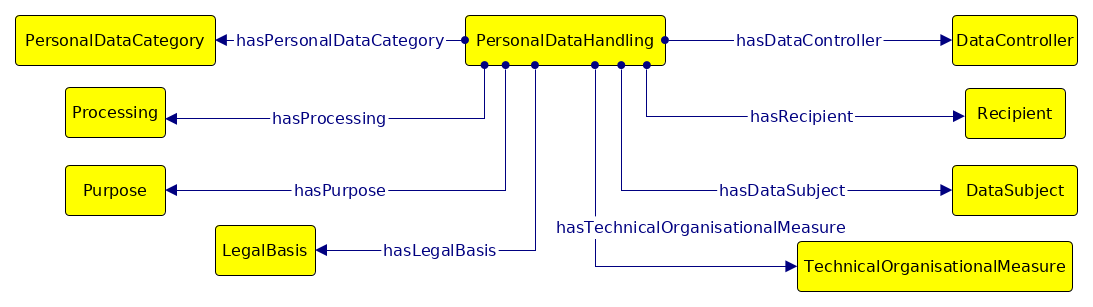
\includegraphics[width=\linewidth]{img/dpv-personaldatahandling.png}
    \caption{Core concepts in DPV \cite{pandit_creating_2019}}
    \label{fig:vocabs:dpv-core}
\end{figure}

\subsubsection{Personal Data Categories}
DPV uses the taxonomy provided by EnterPrivacy\footnote{\url{https://enterprivacy.com/wp-content/uploads/2018/09/Categories-of-Personal-Information.pdf}} to define a broad hierarchy of personal data categories based on nature of information (financial, social, tracking) and to its inherent source (internal, external). 
In addition to these, the class \texttt{dpv:Special\-Category\-Of\-PersonalData} represents categories that are `special' or `sensitive' based on GDPR’s Article 9.

These personal data categories can be further extended using the sub-class mechanism to depict specialised concepts such as `likes regarding movies'.
Sub-classing also enables representation of specific contexts such as derivation of personal data as represented by class \texttt{dpv:DerivedPersonalData}.
This is useful to represent practical representation of personal data categories such as inference of opinions from social media.
Similar classes can be additionally added to specify contexts such as use of machine learning, accuracy, and source.
The aim of providing such high-level concepts is to provide a sufficient coverage of abstract categories of personal data which can be extended using subclass mechanism to represent concepts used in real-world. 

\subsubsection{Purposes}
Purposes in DPV are organised hierarchically using the sub-class mechanism to represent high-level and generic purposes of data handling.
Purposes provided in DPV include service provision, R\&D, commercial interest, security, service optimisation, and service personalisation. These are further extended to provide a total of 31 generic purposes.
These may be extended by further sub-classing to create more specific purposes as applicable to a scenario.
As GDPR requires a specific purpose to be declared in an understandable manner, additional purposes can be created as sub-classes of one or several \texttt{dpv:Purpose} categories to make them as specific in a use-case as possible.
Purposes can be restricted to specific \texttt{contexts} using the class \texttt{dpv:Context} and property \texttt{dpv:hasContext}.
Purposes can also be restricted to a specific \texttt{business sector} using the class \texttt{dpv:Sector} and property \texttt{dpv:hasSector}.

\subsubsection{Processing Categories}
DPV provides a hierarchy of processing categories based on requirements of regulations such as GDPR. 
DPV defines top-level classes to represent following broad categories of processing - Disclose, Copy, Obtain, Remove, Store, Transfer, Transform, and Use.
Each of these are further expanded using sub-classes to provide 33 processing categories, which includes terms defined in definition of processing in GDPR (Article 4-2).
DPV provides properties with a boolean range to indicate nature of processing regarding \texttt{Systematic Monitoring}, \texttt{Evaluation or Scoring}, \texttt{Automated Decision-Making}, \texttt{Matching or Combining}, \texttt{Large Scale processing}, and \texttt{Innovative use of new solutions} - as these affect assessment of legal data processing under GDPR.

\subsubsection{Technical and Organisational Measures}
GDPR Article 32 requires implementing appropriate measures by taking into account state of the art, costs of implementation and - nature, scope, context, and purposes of processing - as well as risks, rights and freedoms.
These are represented as technical and organisational measures in DPV.
Examples include pseudo-anonymisation and encryption of personal data, ability to restore availability and access to personal data in a timely manner in event of a physical or technical incident, and a process for regularly testing, assessing and evaluating effectiveness of technical and organisational measures for ensuring security of processing.
The generic property \texttt{dpv:measureImplementedBy} enables referencing implementation measures as comments or IRIs.
The class \texttt{StorageRestriction} provides expression of measures used for storage of data with two specific properties provided for storage location and duration restrictions.

\subsubsection{Consent and Legal Bases}
DPV provides \texttt{dpv:LegalBasis} as a top-level concept to represent various legal bases that can be used for justifying processing of personal data.
The definition of a `legal basis' is based on justification for processing which has a provision in law. The concept itself is not based on any specific jurisdiction, but needs to be interpreted in terms of legal bases defined and provided by laws applicable within a jurisdiction.

For GDPR, which is a EU specific law and therefore is not binding in interpretation of legal bases across other jurisdiction, DPV provides legal bases specific to GDPR as a separate aligned vocabulary under \url{https://www.w3.org/ns/dpv-gdpr} and namespace (prefix: \texttt{dpv-gdpr}). 
This vocabulary defines legal bases provided by Articles 6 and 9 of GDPR to represent legal justification for processing personal data.

Consent as a special case of legal basis provided by GDPR is provided with additional properties and classes within the core DPV vocabulary to reflect  information requirements associated with its validity as a legal basis.
The concepts associated with consent provide terms to describe consent provision, withdrawal, and expiry.
The structure of these was adapted from an analysis of existing work regarding Consent Receipt \cite{lizar_consent_2017} and GConsent \cite{pandit_gconsent_2019} with the intention to enable documenting attributes associated with consent which can demonstrate and evaluate its validity based on requirements of GDPR.

\subsection{Comparing DPV with GDPRtEXT, GDPRov, and GConsent}
DPV has several commonalities with ontologies presented in this thesis arising from a common aim of representing information for legal compliance with laws such as GDPR.
However, the aim and granularity of representing information about all attributes relevant to processing of personal data differentiates DPV from the scope of ontologies presented in this thesis.
Given the high-level and abstract nature of DPV in its concepts and more granular and representative focus of developed ontologies, there is a possibility of aligning or combining the two based on identifying commonality of concepts.
While there have been no efforts to carry out an exercise to combine or align the developed ontologies with DPV, their comparison as presented here demonstrates the possibility and applicability of such an approach.

\subsubsection{Representing information about GDPR concepts}
GDPRtEXT provides a linked data version of GDPR and a SKOS glossary of concepts associated with GDPR compliance, which can be used to link information to clauses and concepts of GDPR.
This has been used by GDPRov and GConsent to define the source of its concepts within GDPR.

DPV, whose concepts represent generic legal terms, does not link its concepts to GDPR except in cases where a defined concept was directly taken from a definition provided by GDPR.
In such cases, it uses the URI format prescribed by EU Publications Office to indicate specific clause of GDPR. The URI format\footnote{The format is based on using templates to indicate the alphanumeric characters of articles and clauses. The template format can be represented as: \url{https://eur-lex.europa.eu/eli/reg/YEAR/NUMBER/ARTICLE/PARA/POINT/oj}} is similar in its structuring of contents with GDPRtEXT and is based on an upcoming iteration\footnote{The information is based on a private communication between the author of the thesis with members of the EU Publications Office. The prescribed IRI, while not officially published or documented, currently resolves to the web-page of the legislation, which in this case is the GDPR.} of ELI vocabulary which will be used in all EU published legislations to offer granular linking to their clauses.
Since the format prescribed by EU Publications Office is authoritative in its nature, the links provided by GDPRtEXT need to be aligned or replaced with those defined using the newer ELI format.

One of the aims of DPVCG is to provide a glossary of concepts associated with legal personal data handling. For this, concepts of DPV itself are considered a glossary of terms, though not explicitly defined as such within the ontology. This use of `glossary' refers to providing concepts to an adopter in order to represent required information in an interoperable manner. Since these terms do not necessarily arise from a particular legislation, their sources are based on their use as a commonly understood concept or notion within legal domain.

In terms of coverage, GDPRtEXT focuses on terms directly obtained from text of GDPR while DPV focuses on modelling of concepts based on their relevance to defining personal data handling in the legal domain.
Therefore, while there is a small overlap in concepts directly associated with GDPR, the two vocabularies differ in provision and definition of terms. For example, GDPRtEXT defines \texttt{DataSecurity} based on Article 28 and 32 of GDPR as obligations for Controllers and Processors, while DPV defines \texttt{Security} as a purpose. To further exemplify this distinction, DPV aims to offer terms that reflect real-world practices while GDPRtEXT focuses on legal text of GDPR. This is evident from hierarchical taxonomy of concepts in DPV such as for personal data categories and purposes so as to enable modelling of practices across a broader spectrum of use-cases.

\subsubsection{Representing information about activities}
DPV does not provide representation of activities through which it can be compared with GDPRov.
Instead, DPV provides concepts to represent `processes' taking place within an organisation, such as those for ensuring technical and organisational measures, purposes, and processing.
The modelling of an instance of personal data handling, which consists of specifying purpose, processing, and technical \& organisational measures - can be compared with modelling of plans in GDPRov where a purpose represents a plan and its steps represent processing activities - which can be further annotated with measures and legal bases.
Through this, it can be summarised that the focus of GDPRov is on representing activities with granularity in terms of their composition and dependency, and that of DPV is on providing metadata as an overview of  processing and data handling practices. With this, it is possible to define an instance of personal data handling using DPV to indicate a high-level summary and expand it using GDPRov to represent details of processes and capture their provenance in ex-ante/ex-post phases.

\subsubsection{Representing information about consent}
The DPV and GConsent both provide concepts to represent information about consent based on requirements specified by GDPR.
In this, both share an aim to document context of consent with a view towards establishing its validity and compliance.
The difference between the two is based on granularity and use of existing vocabularies to represent this information.

The DPV utilises the model provided by its core or base vocabulary to represent information by specifying consent as a legal basis used to justify processing of personal data.
In addition to this, it provides properties to indicate the specific notice displayed to obtain consent, its expiry, obtaining or provision of consent, and its withdrawal.
In this, attributes such as timestamp and method used to carry out provision and withdrawal are used to indicate information regarding how consent was obtained.
This is based on updating concept from Consent Receipt with requirements of  GDPR.

The DPV does not prescribe or utilise any existing vocabulary to specify information.
In contrast, GConsent provides similar concepts as DPV base vocabulary and uses vocabularies of PROV-O and GDPRov to represent information about activities.
Given that GConsent was an input to DPV and by extension influential in its modelling of consent, there is a degree of compatibility between the two based on similarity of concepts.
In this, GConsent provides a more detailed vocabulary for consent while DPV provides a minimal set of concepts regarding consent but is more expressive in representing information through its taxonomies.

\subsection{Comparing DPV with SotA}\label{sec:voc:dpv-sota}
This sections compares the DPV with approaches presented in the SotA in \autoref{chapter:sota}.
The aim of this exercise to demonstrate extent of DPV's contributions and present its comparison with approaches in SotA.
Since DPV is not presented as a direct contribution of this thesis, its formal evaluation is not within scope of this thesis.

The aim of DPV as established by DPVCG is providing a vocabulary for personal data handling which concerns representation of information relevant for legal compliance - in this case associated with GDPR. Based on this, DPV is a vocabulary useful towards representing information about processing of personal data rather than a framework or methodology that can be used to evaluate compliance.
Currently, DPV is not accompanied by any documentation demonstrating its use or application in use-cases, though such activities are planned in near future.

Comparing DPV with other vocabularies in SotA as presented in \autoref{chapter:sota}, DPV provides a large amount of concepts in its top-down taxonomies which can be expanded with additional concepts. This enables it to be adapted and expanded for use-cases.
This aspect of the DPV is novel within SotA as no other approach aims to provide a similar taxonomy of concepts, and does not incorporate requirements of extending it for a given use-case such as through sub-classing mechanism.

The DPV base vocabulary provides a compact structure representing personal data handling which aims to represent all relevant information required to evaluate and demonstrate compliance.
In this, it bears resemblance to SPECIAL core vocabulary \cite{bonatti_special_2018-2} which is self-explanatory given that DPVCG was an extension of SPECIAL's work on its vocabularies.
This approach is more suitable for representation or documentation of information from a compliance perspective, and is not intended to be specific to any particular law - though the GDPR clearly has a significant influence on its vocabulary.
This is again in contrast to approaches in SotA which are often intended to be applied to a particular legislation and a specific use-case.

The representation of technical and organisational measures is the most distinctive feature of DPV, as currently no other approach within SotA provides a comparable representation of these.
While there have been efforts to establish vocabularies regarding specification and representation of privacy policies, these tend to focus on use of concepts such as purpose, processing, data storage, data sharing, third parties - which have been utilised quite commonly in SotA.

\section*{Chapter Summary}
This chapter presented the ontologies created to fulfil research objective $RO3$ along with the methodology used for their development and evaluation. It also provides a comparison of ontologies with related approaches in SotA as presented in \autoref{chapter:sota}.

The ontology engineering process was presented in \autoref{sec:intro:ontology-engineering} and described the methodology used for creating ontologies based on best-practices and guidelines advocated by semantic web community. This included ensuring ontology quality, documentation, and releasing developed resources under an open and permissive license.
It also described utilisation of compliance questions presented in \autoref{sec:info:compliance-questions} as competency questions.

The presented ontologies consisted of GDPRtEXT, GDPRov, and GConsent.
GDPRtEXT, presented in \autoref{sec:voc:GDPRtEXT}, provides a linked data version of text of GDPR created by extending the official ELI \cite{ELI_2012} ontology to represent GDPR in a granular manner. It also presents a SKOS glossary of concepts associated with GDPR compliance derived from its text. GDPRtEXT enables association and linking of information with concepts and clauses of GDPR through use of persistent IRIs. It thus fulfils research objective $RO3(a)$. GDPRtEXT extends state of the art by providing an ELI-compatible extension capable of representing GDPR clauses at a granular level. It is also novel in providing a glossary of concepts associated with GDPR compliance.

GDPRov provides an OWL2 ontology for representing activities associated with personal data and consent in ex-ante and ex-post phases. It is presented in \autoref{sec:voc:GDPRov}.
The ontology is based on extending existing ontologies of PROV-O \cite{lebo_prov-o_2013} and P-Plan \cite{garijo_p-plan_2014} with GDPR terminology  to represent activities in context of compliance requirements. GDPRov is novel in use of PROV-O and P-Plan together based on a scientific workflow model to represent processes for GDPR compliance.
It provides an extensible model that can be used for representing processes related to compliance which can be extended for representing related  processes such as compliance activities and organisational processes.
Use of GDPRov enables capturing provenance of plans or snapshots of a system at a given time and document them as evidence of planned and maintained compliance.
Use of P-Plan with PROV-O enables associating execution of activities with their intended planning and thereby provides systematic linking of ex-ante and ex-post compliance information.
GDPRov thus fulfils research objective $RO3(b)$.

The representation of consent is provided by GConsent - an OWL2 ontology presented in \autoref{sec:voc:GConsent} that fulfils research objective $RO3(c)$.
GConsent provides representation of information relevant for evaluation of consent under GDPR obligations and requirements.
It extends representation of consent as an artefact in GDPRov and models life-cycle of consent based on the concept of states.
State or status of consent reflects its suitability for use as a legal basis for processing and is modelled based on management of consent information from an organisation's perspective. In this GConsent is novel within SotA.
GConsent is also novel in provision of concepts related to consent for GDPR as it provides a more detailed and comprehensive vocabulary for representing information regarding consent.

The chapter also presented the DPV vocabulary published by W3C Data Privacy and Vocabularies Community Group (DPVCG). The author of the thesis was an active contributor to DPV, and subsequently DPV shares its aim and bears similarity to research presented in this thesis. \autoref{sec:voc:DPV} provides a summary of DPV and compares it with ontologies presented as contributions in this thesis - namely GDPRtEXT, GDPRov, and GConsent. A comparison of DPV with SotA is also provided.
DPV is intended to provide a vocabulary for representing information about personal data handling and is not limited to GDPR though it is influenced by it. It reflects a community consensus and is intended to be standardised, thereby providing a strong basis for its adoption.

Through these developed ontologies and the significance of DPV, the primary motivation guiding this research as outlined at the beginning of this thesis (\autoref{sec:intro:background}) regarding representing information and associating it with GDPR has been addressed.
In the next chapter, use of semantic web technologies to query this information to answer compliance questions, such as those presented in \autoref{sec:info:compliance-questions}, is presented. The next chapter also presents use of semantic web technologies in validating information to ensure its correctness for assessing GDPR compliance based on constraints presented in \autoref{sec:info:constraints}.
The querying and validation of information are minor contributions of this thesis, and satisfy research objectives $RO4$ and $RO5$ respectively.
For this, the next chapter utilises real-world use-cases to demonstrate application of  developed ontologies of GDPRtEXT, GDPRov, and GConsent to represent, query, and validate information for GDPR compliance.
